\documentclass[pra,
aps,
twocolumn,
superscriptaddress,
groupedaddress,
nofootinbib,
reprint
]{revtex4-1}

% PACKAGES
\usepackage{amsmath,amsfonts, amssymb, amsthm}
\usepackage{bm, bbm, physics, mathtools}
\usepackage{graphicx, subfigure}
\usepackage{xcolor, enumerate}
\usepackage{xifthen, hyperref}
\usepackage[capitalise]{cleveref}

\hypersetup{
	colorlinks=true,  
	linkcolor=blue,   
	citecolor=blue,   
	urlcolor=blue     
}

\newcommand{\crefrangeconjunction}{--}
\creflabelformat{figure}{(#2#1#3)}

% COMMENT NOTATION
\newcommand{\nick}[1]{{\color{red}#1}}
\newcommand{\ddd}[1]{\textcolor{blue}{#1}}

% ENVIRONMENTS
\newtheorem{theorem}{Theorem}
\newtheorem{proposition}[theorem]{Proposition}
\newtheorem{lemma}[theorem]{Lemma}
\newtheorem{definition}[theorem]{Definition}

% REFERENCES
\iffalse
\renewcommand{\eqref}[1]{Eq.~(\ref{#1})}
\newcommand{\figref}[1]{Fig.~(\ref{#1})}
\newcommand{\tabref}[1]{Tab.~(\ref{#1})}
\newcommand{\secref}[1]{Section~(\ref{#1})}
\newcommand{\appref}[1]{Appendix~(\ref{#1})}
\newcommand{\defref}[1]{Definition~\ref{#1}}
\newcommand{\lemref}[1]{Lemma~\ref{#1}}
\newcommand{\thmref}[1]{Theorem~\ref{#1}}
\fi

% SYMBOL DEFINITIONS
\renewcommand{\cal}[1]{\mathcal{#1}}

\newcommand{\reals}{\mathbb{R}}
\newcommand{\id}{\mathbbm{1}}
\newcommand{\idc}{1_{\rm{C}}}
\newcommand{\supf}{\mathfrak{c}}
\renewcommand{\tr}{{\rm{tr}}}
\renewcommand{\det}{{\rm{det}}}
\newcommand{\floor}[1]{\left\lfloor #1 \right\rfloor}
\newcommand{\ent}[2]{S\left( #1 \middle\vert\middle\vert #2 \right)}
\newcommand{\ents}{{\ent{\frac{m}{n}}{p}}}

\def\dummy{\ell}
\def\NN{n}
\def\mmf{i}
\def\nnf{n}
\def\mlt{m}
\def\ii{i}
\def\jj{j}
\def\kk{k}
\def\II{I}
\def\nn{n}
\def\tt{n'}
\def\mm{a}
\def\wp{u}
\def\wn{v}

\newcommand{\too}[1]{^{\otimes #1}}
\newcommand{\noisys}{\rho_{\rm{S}}}
\newcommand{\noisysn}{\rho_{\rm{S}}(\epsilon)^{\otimes \nn}}
\newcommand{\noisysN}{\rho_{\rm{S}}(\epsilon)^{\otimes \NN}}

\newcommand{\spanv}[1]{
    {{\rm{span}}\left\{#1\right\}}
}
\newcommand{\conv}[1]{
    {{\rm{conv}}#1}
}
\newcommand{\orb}[1]{
    {{\rm{orb}}(#1)}
}
\newcommand{\sn}[1]{
    {{\rm{sn}}\left(#1\right)}
}
\newcommand{\mana}[1]{
    {{\rm{mana}}\left(#1\right)}
}
\newcommand{\lc}[2]{
	{{\rm{L}}_{#1|#2}}
}

\newcommand{\bmx}{\bm{x}}
\newcommand{\bmy}{\bm{y}}
\newcommand{\bmz}{\bm{z}}
\newcommand{\bmu}{\bm{u}}
\newcommand{\bmw}{\bm{w}}
\newcommand{\bmo}{\bm{0}}
\newcommand{\bmd}{\bm{d}}
\newcommand{\bma}{\bm{a}}
\newcommand{\bmxi}{\bm{\xi}}
\newcommand{\bmg}{\bm{g}}

\newcommand{\zd}[1][]{
    \ifthenelse{\isempty{#1}}{
    {\mathbb{Z}_d} }{
    {\mathbb{Z}_{#1}}}
}
\newcommand{\hd}[1][]{
    \ifthenelse{\isempty{#1}}{
    {\cal{H}_d} }{
    {\cal{H}_{#1}}}
}
\newcommand{\pd}[1][]{
    \ifthenelse{\isempty{#1}}{
    {\cal{P}_d} }{
    {\cal{P}_{#1}}}
}
\newcommand{\cd}[1][]{
    \ifthenelse{\isempty{#1}}{
    {\cal{C}_d} }{
    {\cal{C}_{#1}}}
}
\newcommand{\spd}[1][]{
    \ifthenelse{\isempty{#1}}{
    {{\rm{Sp}}(2, \zd)} }{
    {{\rm{Sp}}(2, \zd[#1])}}
}
\newcommand{\gp}[1][]{
    \ifthenelse{\isempty{#1}}{
    {\rm{GP}_d} }{
    {\rm{GP}_{#1}}}
}
\newcommand{\stoch}[1][]{
    \ifthenelse{\isempty{#1}}{
    {{\rm{S}}_d(\bmd)} }{
    {{\rm{S}}_d(#1)}}
}
\newcommand{\stochw}[1][]{
    \ifthenelse{\isempty{#1}}{
    {{\rm{S}}_{d^2}(\W{\sigma})} }{
    {{\rm{S}}_{d^2}(#1)}}
}
\makeatletter
\def\W{\@ifnextchar[{\@with}{\@without}}
\def\@with[#1]#2{ 
    {{\rm{W}}_{#2}\left(#1\right)} }
\def\@without#1{ 
    {{\rm{W}}_{#1}} }
\makeatother

\newcommand{\T}{\cal{T}}
\newcommand{\Z}{\cal{Z}}

\newcommand{\C}{\cal{C}}
\newcommand{\E}{\cal{E}}
\newcommand{\J}{\cal{J}}
\newcommand{\R}{\cal{R}}
\newcommand{\D}{\cal{D}}
\newcommand{\F}{\cal{F}}
\renewcommand{\O}{\cal{O}}
\newcommand{\M}{\cal{M}}

\newcommand{\Fmax}{\F_{\rm{max}}}
\newcommand{\Omax}{\O_{\rm{}max}}
\newcommand{\Rmax}{\R_{\rm{}max}}
\newcommand{\Pis}{\Pi_{\rm{s}}}
\newcommand{\Pio}{\Pi_{\rm{o}}}

\newcommand{\cptp}{{\rm{CPTP}}}
\newcommand{\cpos}{{\rm{CP}}}
\newcommand{\so}{{\rm{SO}}}
\newcommand{\stab}{{\rm{STAB}}}
\newcommand{\spo}{{\rm{SPO}}}
\newcommand{\cspo}{{\rm{CSPO}}}
\newcommand{\rcu}{{\rm{RCU}}}
\newcommand{\tho}{{\rm{TO}}}
\newcommand{\cpwp}{{\rm{CPWPO}}}
\newcommand{\ru}{{\rm{RU}}}


\begin{document}
% Write bounds as 1 + ln{}/{} or 1 - (-ln{})/{} ?
% Labels and Refs (theorems vs lemmas vs propositions)
% R: rate vs bound ?
% Appendices: clean-up
% Figs check(fig.0, move to app, consistency)

% Notation consistency
% UK vs US english
% Spacing (figs, sections, paragraphs, eq. numbering, \noindent, QEDs)

\begin{abstract}
\ddd{[To be sharpened]} Magic states are key ingredients in schemes to realise universal fault-tolerant quantum computation.
Theories of magic states attempt to quantify this computational element via monotones and determine how these states may be efficiently transformed into useful forms. Here we introduce the concept of `fragments', which generalise the concept of magic monotones and has a natural thermodynamic structure based on majorisation. From this perspective magic can be viewed as a form of free energy within each fragment and is constrained by relative majorisation relations but now on quasi-probability distributions. Notably this approach allows us to incorporate actual physical constraints, for example noise models with particular bias or temperature-dependent features, and study how these constrain general magic distillation protocols. In this context we present general temperature-dependent bounds on distillation rates that any theory of magic must respect. Significantly, this analysis also presents a thermodynamic context which cannot be analysed via traditional methods based on thermodynamic entropies, due to the presence of negativity, and raises novel questions in the context of statistical mechanics.
\end{abstract}

\preprint{APS/123-QED}

\title{General constraints on magic distillation protocols from statistical mechanics}

\author{Nikolaos Koukoulekidis}
	\email{nk2314@imperial.ac.uk}
	\affiliation{Department of Physics, Imperial College London, London SW7 2AZ, UK}
\author{David Jennings}
	\affiliation{School of Physics and Astronomy, University of Leeds, Leeds, LS2 9JT, UK}
	\affiliation{Department of Physics, Imperial College London, London SW7 2AZ, UK}

\date{\today}
\maketitle

%%%%%%%%%%%%%%%%%%%%%%%%%%%%%%%%%%%%%%%%

\section{Introduction}
\label{sec:intro}

\nick{re-write based on new relative majorisation approach}
The past few years have seen rapid progress towards the goal of a fault-tolerant quantum computer~\cite{Fowler_2012, Herrera_2010, Nickerson_2014, Nikahd_2017, chao_2018, lin_pieceable_2020, Lin_2020, Bourassa_2021}. However, many challenges remain and there is increasing need for theory to take into account physical limitations of the hardware involved. The surface code~\cite{Bravyi_1998, Freedman_2001, Dennis_2002, Raussendorf_2007} is a leading framework for fault-tolerance with very high error thresholds. Within this scheme, Clifford unitaries can be implemented in a robust, fault-tolerant way. However, due to the Eastin-Knill theorem~\cite{Eastin_2009}, we also know that it is impossible to have a universal set of transversal gates, and although Clifford unitaries can be realised transversally~\cite{Calderbank_1996, Steane_1996}, one needs to find ways around the Eastin-Knill restriction. This can be achieved by injecting in quantum states, called magic states, which promote the Clifford group to universal quantum computing~\cite{cit:bravyi}. The obstacle to this is that these states are invariably noisy and so protocols involving stabilizer operations must be employed to purify many copies of the magic states and improve the overall performance of the induced quantum gates. A central question then arises about the overhead on purifying many copies of a magic state into less noisy forms. 

To address this, concrete distillation protocols have been developed, such as the Bravyi-Haah protocol that provides a quadratic reduction in noise per cycle~\cite{Bravyi2012}. Such distillation rates have been improved in more recent works~\cite{Hastings2018, Litinski_2019, Krishna2019, cit:prakash}. There is also analysis of magic protocols from the perspective of magic monotones, which provide upper bounds on distillation rates and find application in the analysis of gate synthesis~\cite{Campbell_2017, Howard_2017, Prakash_2018}. These frameworks for magic view magic states as resource states with respect to a natural class of quantum operations that are considered cheap, or free, such as stabilizer operations~\cite{Gour_2019, cit:ahmadi, cit:seddon, Wang_2019}.
  
  
Recent work towards fault-tolerance has begun to bridge the gap between abstract theory and experiment. Extensive work has been done on error mitigation~\cite{Li_2017, Temme_2017, Endo_2018, McClean_2017}, and the incorporation of hardware physics into the theoretical modes~\cite{Kandala_2019, Colless_2018, song2018quantum, Bravyi_2021}. For example, the XZZX code~\cite{bonilla_ataides_xzzx_2021} is a variant of the surface code that incorporates noise bias explicitly and has been shown to attain the hashing bound of random codes~\cite{Bennett_1996}. 

In this work, we develop a framework to analyse magic state distillation protocols where explicit physical constraints are manifest. These physical constraints are encoded in the allowed fixed-point structure of the protocol, for example a minimal temperature attainable in the device, noise-biases or fixed-point structure associated with restricted gate-sets (see e.g.~\cite{Aliferis_2008, Stephens_2013, Li_2015, Babbush_2018, Tuckett_2019, Guillaud_2019, Fowler_2019}). The approach we take is most closely aligned with resource theories of magic, although it differs in two ways. Firstly, we obtain distillation upper bounds without the use of monotones, and secondly our distillation bounds are functions of the physical constraints, thus not directly comparable to global magic monotones.

We approach this problem using tools from statistical mechanics and recent work from the overlap of thermodynamics and quantum information theory~\cite{cit:gour, cit:gour2}\nick{You had a specific review in mind I think, which one?}. In particular, we shall view \emph{magic as a form of free energy}, relative to the set of stabilizer states. This perspective takes the convex set of stabilizer states as the set of ``equilibrium'' states, and magic corresponds to a form of non-equilibrium free energy that is strictly non-classical.

Our analysis relies on the discrete Wigner representation of quantum states, in which all states and operations can be described on a discrete phase space~\cite{Ferrie_2008, Okay_2021}. Crucially, we focus on magic states with negativity in their Wigner representation, which is known to be a necessary condition for universality in the state-injection model~\cite{cit:veitch, cit:mari, cit:gottesman, cit:knill, Campbell_2011}. Interestingly, taking a thermodynamic perspective in this context raises a problem, namely it is impossible to define entropies for quasi-distributions. We circumvent this obstacle by making use of a more fundamental tool in thermodynamics -- majorization theory~\cite{cit:marshall, Veinott_1971, Ruch_1976}. To our knowledge majorization of quasi-distributions has not been considered in quantum physics before, and therefore our analysis is of broader interest to the study of non-classicality in quantum systems.

Our construction provides distillation bounds without relying on magic monotones. Instead of projecting the pre-order of magic states onto the real line (which is what a monotone involves) we instead cover the pre-order of states with a collection of simpler `fragment' pre-orders that admit analysis in terms of majorization. It is this choice of fragment that breaks the equivalence of all stabilizer states in the theory and can be used to consider adding physical constraints in the form of accessible protocols.

Through this approach we obtain a range of upper bounds for magic distillation rates. We provide explicit bounds for magic protocols that generate unital channels, as well as bounds that depend on the temperature and Hamiltonian of the system. We find that the thermodynamics in the presence of negativity is surprisingly non-trivial and displays a range of features that do not appear in classical statistical mechanics. 
Finally, we discuss how our approach could be improved and how it can be exploited to construct explicit lower bounds on distillation that take into account physical structure.

\begin{figure}[t]
    \centering
        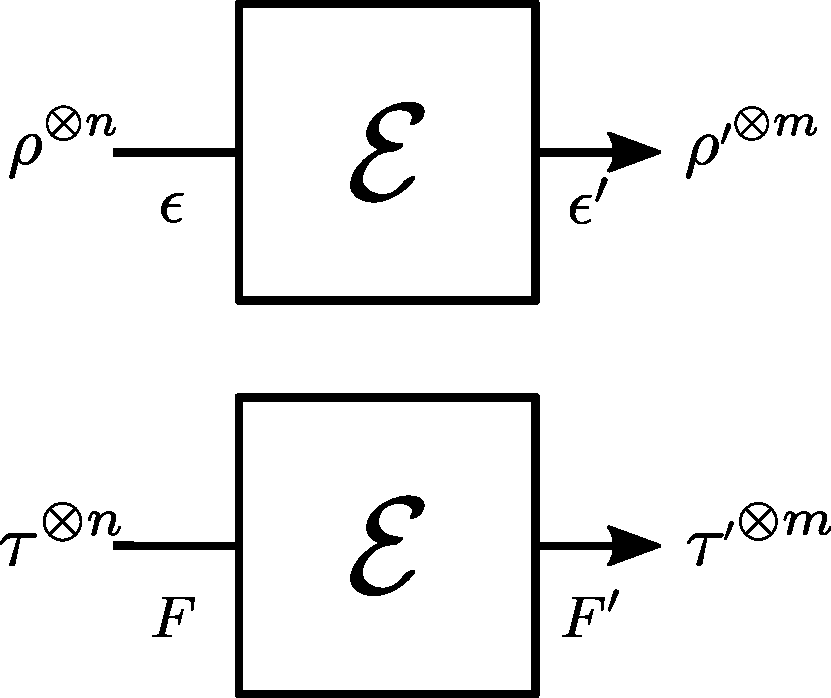
\includegraphics[scale=0.4]{figs/protocol_diagram.pdf}
    \caption{\textbf{Action of a magic protocol} 
	A magic protocol aims to turn $n$ copies of some magic state $\rho_1$ to $m$ copies of some other state $\rho_2$.
	Constraints on the efficiency of the protocol can be imposed by considering its action on an separate probe state $\tau$.
	\nick{How do we improve the illustration?}
    }
    \label{fig:zoo}
\end{figure}

\section{Phase space representations of quantum states}
\label{sec:ps}

Central to our construction is the representation of any quantum state or quantum operation on a system of dimension $d$ in terms of quasi-probability representations on a discrete phase space~\cite{Ferrie_2008}. This construction is a discrete version of Wigner representations in quantum optics~\cite{Wigner_1932, Vourdas_2004}.

Consider a $d$--dimensional quantum system with Hilbert space $\H_d$, and let $\{ |0\>, |1\>, \dots , |d-1\>\}$ denote the standard computational basis, defined over $\mathbb{Z}_d = \{ 0, 1, \dots,d-1 \}$. On this space, generalised Pauli matrices $X, Z$ can be defined by their respective roles as shift and phase operators, acting on the basis states as follows,
\begin{align}
    X \ket{k} &= \ket{k + 1} \label{eq:xpauli}\\
	Z \ket{k} &= \omega^k \ket{k}. \label{eq:zpauli}
\end{align}
Here $\omega \coloneqq e^{2\pi i/d}$ is the $d$-th root of unity and addition is taken modulo $d$. From these we can construct a phase space $\cal{P}_d = \mathbb{Z}_d \times \mathbb{Z}_d$ that provides a complete representation of the quantum system. Given a point $\bmx \coloneqq (x, p)$ we define a displacement operator, 
\begin{equation}\label{eq:ddef}
    D_{\bmx} \coloneqq \tau^{x p} X^{x} Z^{p},\ 
\end{equation}
where the phase factor $\tau \coloneqq -\omega^{1/2}$ ensures unitarity. We assume going forward that $d$ is an odd prime, however the case $d=2$ can also be handled, but with some additional technical caveats~\cite{Appleby_2005}. For a composite system with composite dimension $d = d_1 \dots d_n$ we can decompose the Hilbert space as $\cal{H}_d = \cal{H}_{d_1} \otimes \dots \otimes \cal{H}_{d_n}$, and then define displacement operators as
\begin{equation}\label{eq:composited}
    D_{\bmx} \coloneqq D_{(x_1, p_1)} \otimes \dots \otimes D_{(x_n, p_n)},
\end{equation}
where now we have
\begin{align*}
	\bmx \coloneqq (x_1, p_1, x_2, p_2, \dots, x_n, p_n) \in \cal{P}_{d_1} \times \dots \times \cal{P}_{d_n} \eqqcolon  \cal{P}_d,
\end{align*}
to denote the phase space point for the composite system. 
For simplicity going forward, we assume $n$ copies of a $d$--dimensional system $d_1=d_2 = \cdots = d$, and therefore, we have that $\x \in \mathbb{Z}_d^{2n}$.


The displacement operators form the Heisenberg-Weyl group~\cite{Folland_1989, Bengtsson_2006} under matrix multiplication modulo phases,
\begin{equation}\label{eq:gp}
    {\rm{HW}}_d^n \coloneqq \{ \tau^k D_{\bmx}: k \in \mathbb{Z}_d, \bmx \in \cal{P}_d^n\}.
\end{equation}
The Clifford operations $ \cal{C}_d^n $ are then defined as the set of unitaries that normalise the Heisenberg-Weyl group~\cite{Appleby_2005}. We may define the pure stabiliser states as those states obtained by acting on $|0\>$ with Clifford unitaries~\cite{cit:gross3} and, finally, the full set of stabilizer states as the convex hull of all pure stabilisers, namely all probabilistic mixtures of states of the form $U|0\>\<0|U^\dagger$ where $U$ is Clifford. 

\subsection{Wigner representations for quantum states and quantum operations}\label{sec:wigner}

In order to provide a complete decomposition of arbitrary quantum states and quantum operations we now define a complete basis of Hermitian observables that behaves naturally under the action of the Clifford group. At every point $\x \in \P_d$ we define the phase-point operator
\begin{equation}\label{eq:ax}
	A_{\bmx} \coloneqq \frac{1}{d} \sum_{\bmz \in \cal{P}_d} \omega^{\eta(\bmx, \bmz)} D_{\bmz}, 
\end{equation}
where $\eta(\bmx, \bmz)$ is the symplectic inner product between any two points $\x,\z \in \P_d$, and is given explicitly by
\begin{equation}
	\eta(\bmx, \bmz) \coloneqq \bmz^T \begin{pmatrix}
		0  & \id \\ %\mathbbm{O}_n  & \id_n \\
		-\id & 0 \\ %-\id_n & \mathbbm{O}_n \\
	\end{pmatrix} \bmx,
\end{equation}
where $0, \id$ denote the $n\times n$ zero and identity matrices.

The phase-point operators form an orthogonal operator basis with respect to the Hilbert-Schmidt inner product, as discussed in~\cref{app:wigner}.
Therefore, any quantum state $\rho \in \cal{B}(\cal{H}_d)$ can be expressed as a linear combination of them,
\begin{equation}
    \rho = \sum_{\bmz \in \cal{P}_d} \W[\bmz]{\rho} A_{\bmz},
\end{equation}
where the coefficient vector $\W{\rho}$ is the Wigner distribution of state $\rho$,
\begin{equation}\label{eq:wstate}
    \W[\bmx]{\rho} \coloneqq \frac{1}{d}\tr[A_{\bmx} \rho].
\end{equation}

For any quantum state $\rho$, the Wigner distribution $W_\rho(\bmx)$ is readily seen to be a $d^2$-dimensional quasi-probability distribution over $\cal{P}_d$. More precisely, $W_\rho(\x)$ is a bounded real-valued function on $\P_d$ with the normalisation property $\sum_{\x} W_\rho(\bmx) = 1$ (see~\cref{app:wigner} for details).  In~\cref{fig:wstate_examples}, we show Wigner distributions of different types of qutrit states.

\begin{figure}[t]
    \centering
    \subfigure[][]{%
    \label{fig:maxmix}%
    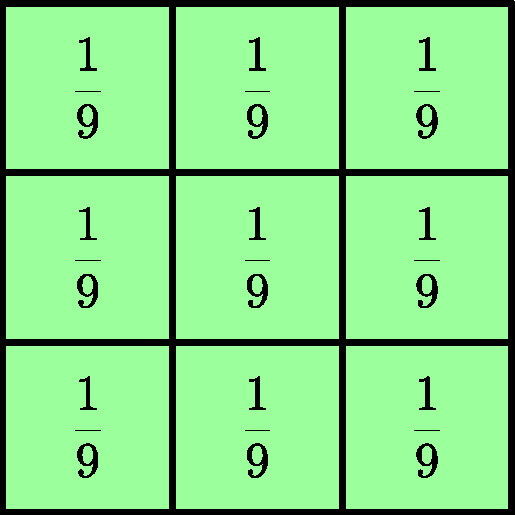
\includegraphics[height=2cm]{figs/maxmixed.pdf}
    %\caption{Maximally mixed state $\frac{1}{3}\id$}%
    }\hspace{8pt}%
    \subfigure[][]{%
    \label{fig:zero}%
    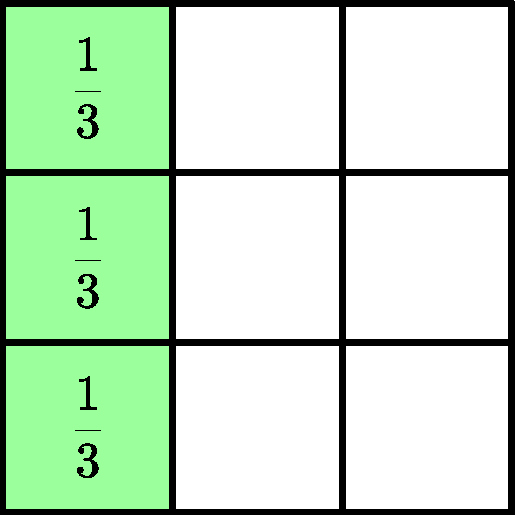
\includegraphics[height=2cm]{figs/zerostate.pdf}
    %\caption{Zero state $\ketbra{0}{0}$}%
    }\\
    \subfigure[][]{%
    \label{fig:bound}%
    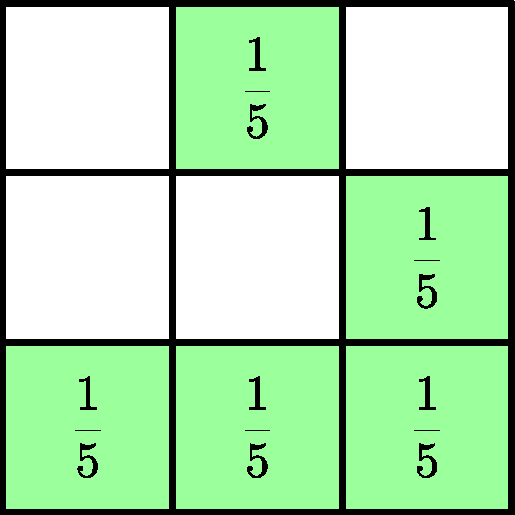
\includegraphics[height=2cm]{figs/boundstate.pdf}
    %\caption{Bound state}%
    }\hspace{8pt}%
    \subfigure[][]{%
    \label{fig:Strange}%
    \includegraphics[height=2cm]{figs/Strangestate.pdf}
    %\caption{Strange state $\ketbra{S}{S}$}%
    }
    \caption{\textbf{Qutrit Wigner distributions of varying magic.} 
    \subref{fig:maxmix} Maximally mixed state $\frac{1}{3}\id$; \subref{fig:zero} Stabilizer zero state $\ketbra{0}{0}$; \subref{fig:bound} A non-stabiliser Wigner-positive state; \subref{fig:Strange} Magic Strange state $\ket{{\rm{S}}} = \frac{1}{\sqrt{2}}(\ket{1} - \ket{2})$, coined in~\cite{cit:veitch2}.
    }%
    \label{fig:wstate_examples}
\end{figure}

Any quantum operation $\E$ can also admit a Wigner representation. If $\E$ maps some quantum system $A$ to a quantum system $B$, and $\J(\E)$ is its associated Choi state then we can define
\begin{equation}
W_{\E}(\y |\x) \coloneqq d_A^2 W_{\J(\E)}(\bar{\x} \oplus \y),
\end{equation}
where $\bar{x} =(x_1, -p_1, \dots , x_n, -p_n)$ can be viewed as the time-reversed version of $\x$ in the discrete phase space, where momenta are reflected while position coordinates remain unchanged.

\subsection{Magic theories for quantum computation}
\label{sec:mono}

A number of magic theories exist, with the central approach of viewing magic states as ``resource'' states with respect to a natural class of quantum operations that are considered free~\cite{Gour_2019}. One very natural class of free operations are those obtained from Clifford operations, measurements and the ability to discard quantum systems. However, there are also other noteworthy candidates~\cite{cit:ahmadi, cit:seddon, Wang_2019}.

In any theory of magic, a natural route to bounding the distillation rates obtainable is through the concept of a \emph{magic monotone}. A magic monotone is a real-valued function of any quantum state $\M(\rho)$ that is monotonically non-increasing under the free operations of the magic theory. More precisely $\M(\sigma) \le \M(\rho)$ whenever it is possible to convert $\rho$ into $\sigma$ using free operations (e.g. Clifford operations).

One of the most prominent magic monotones is the \emph{mana} of a state~\cite{cit:veitch2}, defined as
\begin{equation}
    \mana{\rho} \coloneqq \ln{(2\hspace{1pt}\sn{\rho}+1)},
\end{equation}
where the \emph{sum-negativity}~\cite{cit:veitch2} is the sum of the negative components in $\W{\rho}$,
\begin{equation}
    \sn{\rho} \coloneqq \sum\limits_{\bmx: \W[\bmx]{\rho} < 0} \abs{\W[\bmx]{\rho}}.
\end{equation}

Mana is an additive\footnote{It satisfies the condition $\mana{\rho_1 \otimes \rho_2} = \mana{\rho_1} + \mana{\rho_2}$ which is practical in distillation settings.} magic monotone, so it provides an analytical, necessary condition for many-copy magic state interconvertibility.

A range of monotones have been developed in the literature~\cite{cit:howard, Wang_2020, Seddon_2021} and each provides a means to upper bound distillation rates within a particular theory of magic. In this work we shall develop bounds that apply to essentially any reasonable magic theory. The central idea is to apply majorization theory to the quasi-probability distributions of magic states. In the next section, we explain how these majorization constraints relate to the free operations allowed in a theory of magic.


%%%%%%%%%%%%%%%%%%%%%%%%%%%%%%%%%%%%%%%%

\subsection{Stochastic structure of magic protocols}
\label{sec:struc}

Within the Wigner representation, all negatively represented states are magic states, although in general the converse is not true~\cite{cit:campbell}. However, it is known that all positively represented states used in Clifford circuits admit an efficient classical description, so it is natural to focus on the negatively represented magic states. The free states in any magic theory must therefore lie in the set
\begin{equation}
    \Fmax \coloneqq \{ \rho: \W[\bmx]{\rho} \geq 0 \text{ for all } \bmx \in \cal{P}_d\}.
\end{equation}
Our focus is on states with negativity, so the particular choice of free states is not critical for our analysis. The remaining component that defines any magic theory is the set of allowed quantum operations, i.e. the ones that are considered free. The assumption we require on free operations is simply that they send any free state to another free state, meaning that a resource state cannot be created freely, a common assumption among all magic theories.

We can view the Wigner representation $W_{\E}( \y | \x)$ of a quantum channel $\E$ as a transition matrix mapping points $\x \rightarrow \y$, which is consistent with the representation of quantum states, as
\begin{equation}
	W_{\E(\rho)} (\y) = \sum_{\x \in \P_d} W_{\E}( \y | \x) W_\rho(\x),
\end{equation}
for any $\E$ and $\rho$. Now if $\E$ sends all positively represented quantum state to other positively represented quantum states then it can be shown~\cite{Wang_2019} that $W_{\E}(\y |\x)$ must form a stochastic matrix. In particular, all Clifford operations correspond to stochastic matrices in this Wigner representation. However, it is important to note that not all stochastic maps on the phase space correspond to valid quantum operations. In particular, the stochastic maps must respect the symplectic structure of the phase space, which is an additional non-trivial constraint.

In what follows we shall therefore assume that we have a magic theory $\R = (\F, \O)$ in which the free states $\F$ form a closed set with each state represented by a non-negative Wigner function, while the free operations $\O$ are represented by stochastic maps acting on the discrete phase space.


\section{Magic distillation bounds from majorization theory}
\label{sec:frag}

We wish to consider how physical constraints that may be hardware specific, affect magic distillation rates. These are not a priori encoded in the formulation of the magic theory, and constitute additional physical conditions on top of the underlying resource-theoretic accounting. For example, there may be non-trivial thermal noise in the physical set-up or the accessible operations, there might be strong bias in the noise present, or we might be limited in how easily certain gates can be realised.~\cite{Aliferis_2008, Stephens_2013, Li_2015, Babbush_2018, Tuckett_2019, Guillaud_2019, Fowler_2019}. \nick{repeats intro}

Our formulation will not consider model-specific limitations, but will still inject broad physical constraints. We proceed by considering fixed-point, or ``equilibrium'', restrictions on the actual operations that are accessible to us. While such restrictions could be viewed as the existence of some non-trivial thermodynamic constraint, they could equally be viewed as encoding a high noise-bias or difficulty in realising a particular quantum gate. We can therefore define the following sub-theory of any magic theory $\R$.
\begin{definition}\label{def:sigmafrag}
   Given a theory of magic $\R = (\F, \O)$, the \emph{$\sigma$--fragment of $\R$} is the sub-theory $\R_\sigma = (\F, \O_\sigma)$, in which the free operations are 
   \begin{equation}
        \O_\sigma \coloneqq \{ \E \in \O: \E(\sigma) = \sigma \},
    \end{equation}
namely those operations that leave the state $\sigma \in \F$ invariant.
\end{definition}
This notion provides a simple way to break up any theory into smaller, more manageable parts that are destinguished by additional physical constraints, illustrated in~\cref{fig:zoo}. Moreover, the union over all fragments returns the parent theory, so we are not discarding any information by breaking up the theory in this way. We make this statement precise as follows.
\begin{theorem}\label{thm:frag}
    Let $\R = (\F, \O)$ be a theory of magic.
Then a transformation $\rho \longrightarrow \tau$ is possible in $\R$ if and only if the transformation $\rho \longrightarrow \tau$ is possible in at least one $\sigma$--fragment of $\R$.
\end{theorem}
\begin{proof}
	The proof is straightforward.
   Suppose the interconversion is possible in a $\sigma$--fragment via some $\E \in \O_\sigma$. But since $\O_\sigma \subseteq \O$ it is also possible in $\R$. Conversely, suppose the transformation is possible in $\R$ via some $\E$ in $\O$. The free states $\F$ are a closed, bounded set and moreover the image of $\F$ under the map $\E$ is in $\F$. By the Brouwer Fixed-Point theorem~\cite{cit:brouwer} this mapping must therefore have a fixed point $\sigma \in \F$. Therefore $\E \in \O_\sigma$ and so the interconversion is possible in this fragment.
\end{proof}

\begin{figure}[t]
    \centering
        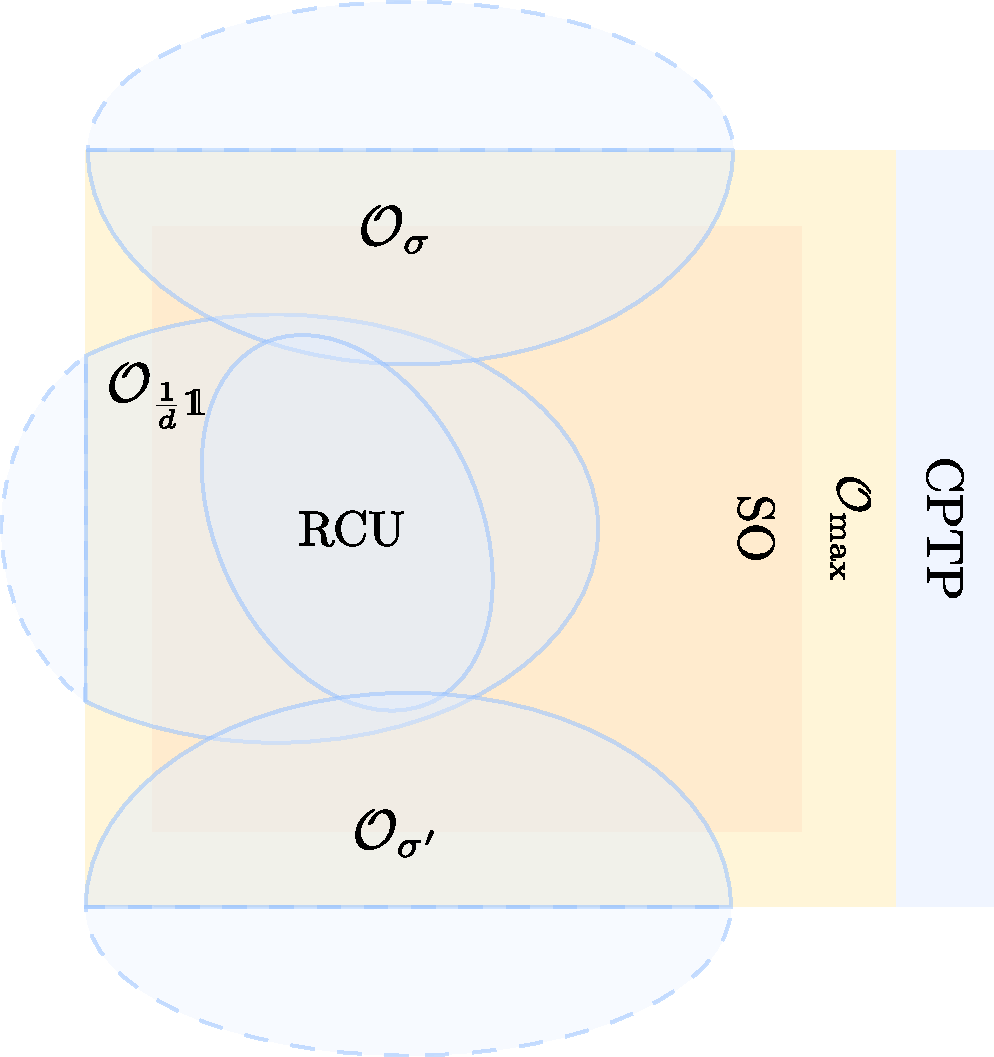
\includegraphics[scale=0.3]{figs/operations.pdf}
    \caption{\textbf{Decomposition of a magic theory $\R$ into $\sigma$--fragments.} 
	Examples of magic theories ($\so$: Stabilizer operations, $\Omax$: Completely positive-Wigner-preserving operations, $\rcu$: Random Clifford Unitaries -- subclass of $\so$) are labelled, with other established magic theories also contained within the yellow regions.
    We introduce $\sigma$--fragments $\O_\sigma$ defined for all free states $\sigma$ that cover $\Omax$. 
    Each $\O_\sigma$ is extensible to a set of stochastic maps outside the $\cptp$ operations.
    Within each $\sigma$--fragment, relative majorisation can be used allowing for a tractable approach towards the study of magic state interconversions.
    }
    \label{fig:zoo}
\end{figure}

It is now possible to consider magic distillation rates within $\sigma$--fragments and then see how the bounds on the distillation rates depend on the choice of the fragment we work within. Therefore, this route can potentially shed light on how the physics of a protocol constrain distillation rates above and beyond global constraints from the parent resource theory. For example, how does temperature affect distillation bounds? Do isotropic maps have better bounds, or does bias towards some pure stabilizer state provide more freedom?
\nick{re-write based on new relative majorisation approach}

By introducing this additional structure to a magic theory, we allow for deeper analysis than would be possible at the level of the full parent theory. In particular, the interconversion structure in each fragment can be analysed using tools from single-shot thermodynamics and majorization theory as we discuss in the next section.

\subsection{Quantifying disorder without entropies}
\label{sec:major}

We can now show that each magic fragment admits constraints that do not take the form of state monotones. 

The question is now whether the sub-theories can be analysed to provide additional insights into magic distillation protocols. An answer can be provided by working in the Wigner representation of a given $\sigma$--fragment. The problem of magic state distillation then becomes that of processing negativity under stochastic maps $W_{\E}( \y |\x)$ that leave a particular quasi-distribution $W_\sigma(\x)$ invariant. However, $\sigma \in \F$ is positively represented, so the sub-theory has an invariant classical probability distribution as a fixed point. This structure allows us to make use of a range of classical tools, and in particular majorization theory.

Majorisation is a collection of powerful tools that has recently found many applications in quantum information theory~\cite{Nielsen_1999, cit:cwiklinski, cit:lostaglio2, cit:gour, cit:gour2, Horodecki_2003, Vallejos_2021}.
It describes the disorder of distributions that undergo stochastic transformations. In its simplest form it defines a pre-order on probability distributions. Given two distributions $\p= (p_1, \dots, p_n)$ and $\q = (q_1, \dots, q_n)$ over $n$ outcomes, we say that $\p$ majorises $\q$, denoted $\p \succ \q$, if there exists a bistochastic map $A = (A_{ij})$ such that $A\p = \q$, where bistochastic means that $A_{ij} \geq 0$ and $\sum_i A_{ij} = \sum_j A_{ij} = 1$. A well-known result~\cite{cit:marshall} tells us that the condition $ \p \succ \q$ over probability distributions is equivalent to $n-1$ inequalities, which can be checked efficiently.

There is a natural generalisation, which is called $\bmd$--majorization~\cite{Veinott_1971}, or in the context of thermodynamics, thermo-majorization~\cite{cit:horodecki2013}. For a fixed probability distribution $\r = (r_1, \dots, r_n)$ with positive components, we define majorization relative to $\r$ as $\p \succ_{\r} \q$, if and only if there exists a stochastic map $A$ such that $A\r = \r$ and $A \p = \q$. In order words, this majorization pre-order coincides with the image of $\p$ under stochastic maps that have $\r$ as a fixed point. It is readily checked that the original majorization condition between probability distributions corresponds to the case $\r = (1/n, \dots, 1/n)$. The pre-order that results from relative majorization is also easily checked and again corresponds to checking a small number of inequalities.

We can further generalise this to \emph{relative majorization}~\cite{Ruch_1976, ruch_mixing_1978, Renes_2016, Buscemi_2017}, defined as an ordering between pairs of vectors so that 
\begin{equation}
	(\p,\r) \succ (\q, \r')
\end{equation}
iff there is a stochastic map $A$ such that $A\r = \r'$ and $A\p = \q$. We retrieve $\bmd$--majorization when $\r = \r'$.

It turns out that relative majorization is equally applicable to \emph{quasi-probability} distributions, and therefore can be applied to the Wigner representation of magic across fragments. We go into more detail on this in the next section.

\subsection{Quasi-probability majorization and non-monotonic Lorenz curves}
\label{sec:lc}

We wish to apply majorization to describing magic in different fragments at the level of the associated Wigner distributions. However, these are in general quasi-probability distributions and so it is important to detail how majorization is computed for these cases and what differences quasi-distributions bring over genuine probability distributions.

Central to the analysis is the notion of a Lorenz curve of a vector $\w \in \mathbb{R}^n$ relative to some other vector $\r \in \mathbb{R}^n$. Given a vector $\w$ we define $\w^\downarrow$ to be the re-arrangement of the components of $\w$ into decreasing order. Given two $n$--component vectors $\w$ and $\r$, we first define $\widetilde{\w}$, where $\widetilde{w}_i \coloneqq w_i/r_i$, as the vector of component-wise ratios between $\w$ and $\r$.
We can now define the \emph{Lorenz curve} of $\w$ relative to $\r$, denoted $L_{\w|\r}(x)$, as the piece-wise linear function that passes through $(0,0)$ and the $n$ points
\begin{equation}
\label{eq:lc}
        (x_k,L_{\w|\r}(x_k)) =\left( \frac{1}{R}\sum_{i=1}^k r_{\pi(i)}, \sum_{i=1}^k w_{\pi(i)} \right),
\end{equation}
where $R\coloneqq \sum_{i=1}^n r_i$ and $\pi$ is the permutation on $n$ objects mapping $\widetilde{\w}$ to $\widetilde{\w}^{\downarrow}$. The form of this requires that $\r$ has no zero components, which we shall assume without loss of generality as in any physical situation the rank of a quantum state is not an operationally meaningful quantity.
We also observe that the curve contains non-differentiable points, called \emph{elbows} at locations where $\widetilde{\bmw}$ changes value.

If $\w$ and $\r$ are both probability distributions then the Lorenz curve is defined on the interval $[0,1]$, and rises monotonically until it reaches the value $1$ at $x=1$. The value $L_{\w|\r}(x) = 1$ is a global maximum, attained at the end-point $x=1$. Moreover, if $\w, \w', \r, \r'$ are all valid probability distributions with neither of $\r,\r'$ having negative components then it has been shown in~\cite{ruch_mixing_1978} that
\begin{equation}
(\w, \r) \succ (\w', \r') \mbox{ if and only if } L_{\w |\r}(x) \ge L_{\w' |\r'}(x).
\end{equation}
This provides a simple way of computing whether relative majorization holds between pairs of probability distributions.

However, if $\w$ is a \emph{quasi-probability} distribution with negative values, and $\r$ a regular probability distribution things are different. Now the Lorenz curve is no longer monotone increasing, but is a concave function that breaks through the $L_{\w|\r}(x) = 1$ barrier at an interior point and attains some non-trivial maximum $L_\star$ above the value $1$, before decreasing monotonically to $L_{\w|\r}(x)= 1$ at the end-point $x=1$. See Figure \ref{fig:lcs} for examples of non-monotonic Lorenz curves for quasi-distributions. Within quantum theory, the breaking of this barrier is associated with the degree of non-classicality. Since majorization provides a measure of order/disorder this is consistent with the intuition that negativity, for example within the context of entanglement theory or quantum computing, can provide a greater form of order than is possible within classical theory.

\begin{figure}
    \centering
    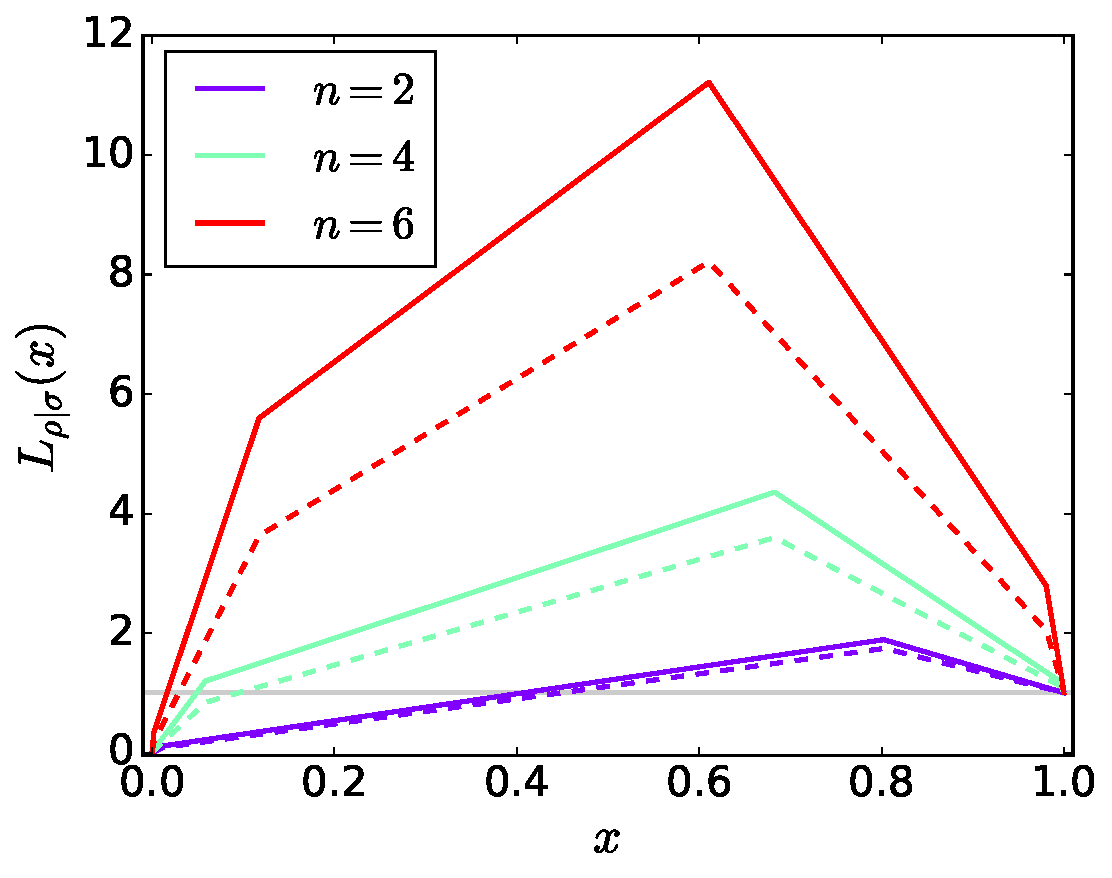
\includegraphics[scale=0.35]{figs/lc_strange.pdf}
    \caption{\textbf{A `heretical' family of Lorenz curves.} Traditionally, Lorenz curves for distributions are monotone increasing cumulant functions that reach a maximum value of $1$. In contrast, Lorenz curves for magic states break through the value of $L(x)=1$ due to the presence of negativity in the associated quasi-probability distributions. The above family of curves correspond to multiple copies of noisy Strange states $\rho\coloneqq\rho_{\rm{S}}(\epsilon)^{\otimes n}$ (\cref{eq:noisysn}) for $n=2,4,6$ within a particular stabilizer fragment ($\sigma = \id/3$). Solid lines represent pure Strange states, while dashed lines represent $\epsilon$-noisy Strange states with depolarising noise $\epsilon = 0.1$.
    }
    \label{fig:lcs}
\end{figure}

However, relative majorization is usually considered for probability distributions, so we need to verify that the same Lorenz curve conditions apply to quasi-probability distributions before proceeding with our analysis. This can be done from first principles, but a simpler way is see that this holds is to reduce to the problem of genuine distributions by first `masking' the negativity in the quasi-probability distribution $\w$ using the reference distribution $\r$ and then applying the conditions for relative majorization. 
 
More precisely, since the components of $\r$ are strictly positive, there always exists an $\epsilon >0$ such that $\w_\epsilon \coloneqq \epsilon \w + (1-\epsilon) \r$ is a genuine probability distribution. We can see that $(\w , \r) \succ (\w', \r')$ if and only if $(\w_\epsilon , \r) \succ (\w_\epsilon', \r')$, where we choose $\epsilon$ so that both $\w_\epsilon$ and $\w_\epsilon'$ are probability distributions. This equivalence holds because there exists a stochastic map $A$ such that $A \w = \w'$ and $A \r = \r'$ if and only if 
\begin{equation}
A[\epsilon \w + (1-\epsilon) \r] = \epsilon \w' + (1-\epsilon) \r'\mbox{ and } A\r = \r'.
\end{equation}
As mentioned, relative majorization between pairs of distributions occurs if and only if the associated Lorenz curves never cross. Therefore, we can express this condition in terms of the Lorenz curves of the quasi-probability distributions $\w$ and $\w'$ relative to $\r$ and $\r'$ respectively.

As shown in Appendix \ref{lemma:Lorenz_linearity}, the Lorenz curve for any quasi-probability distribution obeys the following linearity condition
\begin{equation}
L_{a \w + b \r | \r} (x) = a L_{\w|\r} (x) + bx,
\end{equation}
for all $a >0$ and any $b \in \mathbb{R}$. We now have that
\begin{equation}
(\w, \r) \succ (\w', \r') \mbox{ if and only if } (\w_\epsilon , \r) \succ (\w_\epsilon', \r'),
\end{equation}
and also $(\w_\epsilon , \r) \succ (\w_\epsilon', \r')$ if and only if $L_{\w_\epsilon |\r} (x) \ge L_{\w'_\epsilon |\r'} (x)$ for all $x$. However, using the above linearity property of the Lorenz curves we have that
\begin{align}
L_{\w_\epsilon |\r} (x) &\ge L_{\w'_\epsilon |\r'} (x) \nonumber \\ 
&\mbox{ if and only if }& \nonumber \\
\epsilon L_{\w |\r} (x) + (1-\epsilon) x &\ge \epsilon L_{\w' |\r'} (x) + (1-\epsilon) x.
\end{align}
The $(1-\epsilon)$ terms cancel on both sides and we get the required relative majorization conditions for the quasi-distributions in terms of their Lorenz curves.

We therefore have that $(\w, \r) \succ (\w', \r')$ if and only if $L_{\w | \r} (x) \ge L_{\w' | \r'}(x)$ for all $x \in [0,1]$ equally applies for the case of $\w,\w'$ being quasi-distributions. 

In the next section we discuss the application of majorization to Wigner representations of magic, where the quasi-distribution $W_\rho(x)$ of a magic state can be analysed relative to any Wigner positive free state $W_\sigma(x)$. To our knowledge, the application of majorization to quasi-distributions in  physics has not been considered previously. The caveat here is that relative majorization ranges over stochastic maps that obey a transformation ($A\r = \r'$), while in the case of the Wigner representation there is a stronger restriction that the symplectic structure of the phase space is respected. Therefore, any majorization constraint can provide necessary, but not sufficient conditions on magic state interconversions. This observation raises a question that to our knowledge has not been previously considered in the classical statistical mechanics literature: what are the conditions for symplectic majorization of classical statistical mechanics? We shall return to this question later on when we discuss how our approach could be used to construct concrete lower-bounds on distillation rates in~\cref{sec:lower_bounds}.

\subsection{Majorisation of negative Wigner distributions within $\sigma$--fragments}
\label{sec:major_frag}

Having described how majorization relative to a fiducial distribution can be computed, we now turn to its application within a particular fragment of a magic theory $\R= (\F, \O)$.

If we consider some $\sigma \in \F$, and its corresponding fragment $\R_\sigma$, then we are typically interested in the ability to transform many copies of some magic state $\rho$ into more pure forms of magic. The state $\rho$ is assumed to have negativity in the Wigner representation, so $W_\rho(\x) < 0$ for some regions of $\x \in \P_d$. We again note that we restrict to odd-dimensional quantum systems, for simplicity. In contrast, the state $\sigma$ will have a Wigner distribution $W_\sigma(\x)$ that forms a genuine probability distribution. On the technical assumption that $\sigma$ is full rank, we also have that $W_\sigma(\x) > 0$ for all $\x \in \P_d$. Any non-full rank states $\sigma$ can be handled as a limiting case in which we inject an infinitesimal fraction of depolarising noise $\epsilon (\id/d)$.

As discussed already, the free operations within the magic theory $\R$ are represented by stochastic maps, and within $\R_\sigma$ by stochastic maps that leave $W_\sigma(\x)$ invariant. Therefore, a necessary condition for magic state transformations $\rho_1 \rightarrow \rho_2$ within $\R_\sigma$ will be that 
\begin{equation}
	W_{\rho_1} \succ_{W_{\sigma}} W_{\rho_2},
\end{equation}
or put another way, that the quasi-distribution $W_{\rho_1}$ is more ordered than the quasi-distribution $W_{\rho_2}$ relative to $W_\sigma$.

This in turn can be expressed in terms of Lorenz curves. To simplify notation, we denote by $L_{\rho | \sigma}(x)$ the Lorenz curve $L_{W_{\rho} | W_{\sigma}} (x)$. We therefore have that
\begin{equation}
\rho_1 \rightarrow \rho_2 \mbox{ within }\R_\sigma \mbox{ implies } L_{\rho_1 |\sigma} (x) \ge L_{\rho_2 |\sigma} (x),
\end{equation}
for all $x \in [0,1]$. Therefore, the magic state Lorenz curve condition can be used to impose upper bounds on magic distillation rates. Note, however, that unlike any monotone, this is not a single numerical constraint, but a \emph{family} of constraints. Indeed, for $n$ copies of a $d$--dimensional system the number of terms in $W_{\rho}$ is $d^{2n}$, so the Lorenz curve condition corresponds to exponentially many constraints, of which though there are at most as many independent constraints as there are elbows in the Lorenz curve of the output state, as proved in~\cref{thm:elbows} of~\cref{app:frag}.
In principle, any one location $x$ provides some valid constraint leading to an upper distillation bound, while optimising over the location provides the strictest majorisation bound.

\subsection{Basic monotones for magic states in a particular fragment}
\label{sec:monotones_frag}

In this section, we give some generic aspects of Lorenz curves for magic states. In particular, these allow us to interpret previous magic monotones in a new light. The first result provides an extremely simple way to see that the sum-negativity of a magic state is a monotone.

\begin{lemma} Relative majorization in any fragment implies the monotonicity of sum-negativity. 
\end{lemma}
\begin{proof}
	The sum-negativity of a magic state $\rho$ can be written as $sn(\rho) \coloneqq \frac{1}{2} (\sum_{\x} |W_\rho(\x) | - 1)$.
We make use of a variant form of relative majorization, (see~\cref{app:major}), stating that $\p \succ_{\r} \q$ if and only if
	\begin{equation}
\sum_k | p_k - r_k t | \geq \sum_k | q_k - r_k t |,
\end{equation}
for all $t\in \mathbb{R}$. Choosing $t=0$ we get the single condition that $\sum_k |p_k| \ge |\sum_k |q_k|$, independent of the choice of $\r$. Applying this to the Wigner quasi-distributions of two quantum states immediately gives the result.
\end{proof}
As a corollary, this result applies to mana too, since mana is an increasing function of sum-negativity.

If we have a magic state $\rho$ that has negativity in its Wigner representation, then, as discussed, its Lorenz curve over-shoots $1$ and reaches a non-trivial maximum $L_\star$ that depends on the particular state. There is an exact relation between $L_\star$ and sum-negativity or mana, which is provided by the following result. 
\begin{theorem}\label{lem:lcmax}
	Given a magic state $\rho$, the maximum $L_\star$ of its Lorenz curve $\lc{\rho}{\sigma}(x)$ is independent of the $\sigma$--fragment and equal to $1+\sn{\rho}$. Moreover, the majorization constraint is stronger than mana in every fragment.
\end{theorem}
The proof of this is given in~\cref{app:major}. Using the Lorenz curve perspective, it is simple to construct other monotones. For example, within a given fragment, the area above $L=1$ is another magic monotone.
\begin{lemma}
Given a magic state $\rho$ and a free state $\sigma$, let $\A_\sigma(\rho)$ be the area of the region $\{(x, y): 1 \leq y \leq L_{\rho | \sigma}(x)\}$. Then $\A_\sigma(\rho)$ is a magic monotone for $\R_\sigma$.
\end{lemma}
\begin{proof}
Consider the transformation $\rho_1 \rightarrow \rho_2$ within $\R_\sigma$. We have that $L_{\rho_1|\sigma}(x)$ is never below the curve $L_{\rho_2|\sigma}(x)$, and therefore the region above $L=1$ for $\rho_2$ is a subset of the corresponding region for $\rho_1$. Thus, $\A_\sigma(\rho_1) \geq \A_\sigma(\rho_2)$, so $\A_\sigma$ is a magic monotone in $\R_\sigma$.
\end{proof}
In contrast to mana, the area monotone is \emph{specific to the fragment}, and its value will vary as we change $\sigma$. Therefore its monotonicity is also including the physics of the fragment and provides a means to analyse magic distillation only under free operations that leave $\sigma$ invariant.

We ultimately want to make statements about asymptotic distillation rates $R$,
\begin{equation}
\rho_1^{\otimes n} \longrightarrow \rho_2^{\otimes R n}
\end{equation}
where $\rho_2$ is a purer magic state than $\rho_1$ and $R$ is made as large as possible as $n$ tends to infinity. We shall next turn to this analysis, and exploit basic features of a magic state in order to obtain non-trivial distillation bounds.

\subsection{Magic bounds for unital protocols}
\label{sec:unital}

In this section, we apply majorization to magic state distillation within a simple fragment, namely the unital fragment. This encompasses distillation protocols where one is restricted to \emph{unital operations}, meaning that $\E(\I/d) = \I/d$ for all free $\E$. This is a particularly powerful set of operations, which for example include all Weyl-covariant channels~\cite{cit:gross3}. To make things concrete, we shall consider qutrit magic states ($d=3$) as the Wigner representation is simpler compared to qubits ($d=2$), while they admit non-trivial structure (e.g. Hamiltonians with two different energy gaps) and still are sufficiently simple to analyse in detail.

For our distillation protocols we need to choose a canonical pure magic state as a target. For this we shall choose the Strange state $|S\>$ given as
\begin{equation}
|S\> \coloneqq \frac{1}{\sqrt{2}} (|1\> + |2\>),
\end{equation}
in the computational basis. This qutrit magic state is exceptionally symmetric and simple which benefits our analysis. Its distribution $W_S(\x)$ has a single negative value of $-1/3$ at $\x =(0,0)$ and the positive value $1/6$ at all other points. We can define the $\epsilon$--noisy Strange state as
\begin{equation}\label{eq:noisysn}
    \rho_{\rm{S}}(\epsilon)\coloneqq (1 - \epsilon) \ket{\rm{S}}\bra{\rm{S}} + \epsilon \frac{1}{3}\id,
\end{equation}
where $\epsilon$ is the depolarization noise parameter. Moreover, utilising the symmetries of the Strange state allow for any magic state $\rho$ to be processed via Clifford operations~\cite{cit:prakash,cit:prakash2} and put into this canonical form for some $\epsilon \ge 0$.

The Wigner distribution of the single-copy, $\epsilon$--noisy Strange state  is given by
\begin{equation}
	\W[\bmx]{\rho_{\rm{S}}(\epsilon)} = (1-\epsilon)\W[\bmx]{\ketbra{\rm{S}}} + \epsilon\W[\bmx]{\frac{1}{3}\id}.
\end{equation}
Since the Wigner distribution $W_{\I/3}(x)$ is the uniform probability distribution over the phase space, we get that $W_{\rho_S(\epsilon) } (\x)$ has a single negative component
\begin{equation}
	- v(\epsilon) \coloneqq - \left( \frac{1}{3} -\frac{4}{9}\epsilon \right)
\end{equation} 
located at the origin $\bmx = \bmo$ and positive components
\begin{equation}
	u(\epsilon) \coloneqq \frac{1}{6} -\frac{1}{18}\epsilon
\end{equation}
at the 8 phase space points $\x \ne (0,0)$. We assume that $\epsilon < 3/4$ to ensure the presence of negativity in the Wigner distribution. 

We now consider the task of purifying $n$ copies of a noisy Strange state $\rho_{\rm{S}}(\epsilon)^{\otimes n}$ as given in~\cref{eq:noisysn} into a smaller number of copies $n'$ of a less noisy Strange state $\rho_{\rm{S}}(\epsilon')^{\otimes n'}$, with $\epsilon' < \epsilon$ and $n' \leq n$. Since we work in the unital fragment, the maximally mixed state is free and we choose to tensor in $n'-n$ auxiliary copies of it to the output, highlighting that we are working in the unital fragment. This affects neither the distillation process nor our analysis, since the Lorenz curves remain unaffected. More generally, it is easy to see that
\begin{equation}
	L_{\rho |\sigma} (x) = L_{\rho \otimes \sigma |\sigma \otimes \sigma}(x),
\end{equation}
for any full-rank $\sigma \in \F$. Therefore, we consider the transformation
\begin{equation}\label{eq:sudist}
	\rho_{\rm{S}}(\epsilon)^{\otimes n} \longrightarrow \rho_{\rm{S}}(\epsilon')^{\otimes n'} \otimes \left( \frac{1}{3}\id \right)^{\otimes (n-n')},
\end{equation}
and compare the Lorenz curves for the input and output states to bound $R(\epsilon, \epsilon') \coloneqq n'/n$, the rate of this interconversion within the fragment.

The Wigner distribution of $n$ copies of the state is obtained by the $n$-fold product of the single copy distribution, and the Lorenz curve $L_{\rho|\sigma}(x)$ for $\rho = \rho_S(\epsilon)^{\otimes n}$ and $\sigma = (\I/3)^{\otimes n}$ is readily computed for any $n$ and $\epsilon$, and the full details are provided in~\cref{app:lcsu_technical}.
We highlight that the non-trivial element that arises for quasi-distributions is that the product of negative components can generate a positive $n$-fold component, so the ordering of the components of \emph{rescaled Wigner distribution} $W_{\rho |\sigma}(\bmx) \coloneqq W_{\rho}(\bmx)/W_{\sigma}(\bmx)$ depends on whether $-v(\epsilon)$ appears to an even or odd power in the expression of~\cref{eq:wigu}.

The component values $w_i$ and associated multiplicities ($m_i$) in the $n$--copy case are 
\begin{align}
	m_i &= 8^{i}\binom{n}{i}, \\
	w_i &= u^{i}(-v)^{n-i}, \label{eq:wigu}
\end{align}
where index $i$ runs through $0, \dots, n$, and we assume for simplicity of exposition that $n$ is even and the noise level is not high, $\epsilon \leq 3/7$, so that $v \geq u$.
The details of this scenario, along with the other possible cases that occur depending on the noise level and the parity of the number of copies, are provided in~\cref{app:lcsu_technical}.

The Lorenz curve $L_{\rho|\sigma}(x)$ rises monotonically and reaches a maximum value
\begin{align}\label{eq:lcsu_max}
	L_\star &\coloneqq L_{\rho |\sigma} (x_\star) = \sum_{i = 0}^{n/2} m_{2i} w_{2i} \nonumber\\
	&= \frac{1}{2} + \frac{1}{2}\left(\frac{15 - 8\epsilon}{9}\right)^n > 1,
\end{align}
which occurs at $x=x_\star$ given by
\begin{equation}
	x_\star = \frac{1}{2} + \frac{1}{2}\left(\frac{7}{9}\right)^n.
\end{equation}

It is possible to derive distillation bounds from any location of the Lorenz curve, including the region around the peak, by imposing the constraint that the Lorenz curve of the input state never dips below the curve of the output.
However, it turns out that a simple and sufficiently non-trivial constraint can be obtained by considering the first elbow of the Lorenz curves. 
The largest Wigner component occurs for $i=0$ and is unique, so the first elbow coordinates for $\rho_S(\epsilon)^{\otimes n}$ are given by $(1/9^n, v(\epsilon)^n)$, while for $\rho_S(\epsilon')^{\otimes n'}$ by $(1/9^{n'}, v(\epsilon')^{n'})$.

The first elbow constraint involves a simple interpolation, done in~\cref{app:elb_constraints}, in order to find the coordinates of both Lorenz curve points at the location where the first elbow occurs. 
Comparing these two points leads to the bound
\begin{equation}
	R(\epsilon, \epsilon') \leq \frac{\ln{(3-4\epsilon)}}{\ln{(3-4\epsilon')}}.
\end{equation}
For the limiting case of distilling pure magic states ($\epsilon'=0$), we obtain an upper bound in the unital fragment given by
\begin{equation}
	R \leq 1 + \frac{\ln (1 - \frac{4}{3} \epsilon)}{\ln 3}.
\end{equation}

Similar upper bounds on distillation rates for qudits of odd prime dimension include the mana bound~\cite{cit:veitch} and the max--thauma bound~\cite{Wang_2020} which can be defined as
\begin{equation}
	\theta_{\rm{max}}(\rho) \coloneqq \log_2{\min{\{2\hspace{1pt}\sn{V}+1 : V \geq \rho\}}}
\end{equation}
and can be calculated numerically via a semi-definite program\footnote{Provided as supplemental material with~\cite{Wang_2020}}.

The mana bound can be directly calculated as
\begin{equation}
	R \leq \frac{\mana{\rho_{\rm{S}}(\epsilon)}}{\mana{\rho_{\rm{S}}(0)}} = 1 + \frac{\ln \left(1 - \frac{8}{15}\epsilon \right)}{\ln \frac{5}{3}}.
\end{equation}
For the noisy Strange state, the max--thauma bound coincides with the mana bound, and are both looser than the majorization bound we derived via the first elbow constraint as illustrated in~\cref{fig:distill_bounds}. 
Numerical, ``optimal'', bounds $R_{\rm{opt}}$ obtained by considering the entirety of the Lorenz curves have been included in the plot as well, highlighting that the first elbow constraint does not capture the full capabilities of majorization.
Notably, in contrast to the other bounds, $R_{\rm{opt}}$ depends explicitly on the copies $m,n$, rather than their ratio $m/n$, so it is specific to the process.
An interesting open question arises regarding the value of $R_{\rm{opt}}$ as $n,m \rightarrow \infty$, while $m/n$ remains constant.
\begin{figure}[t]
    \centering
    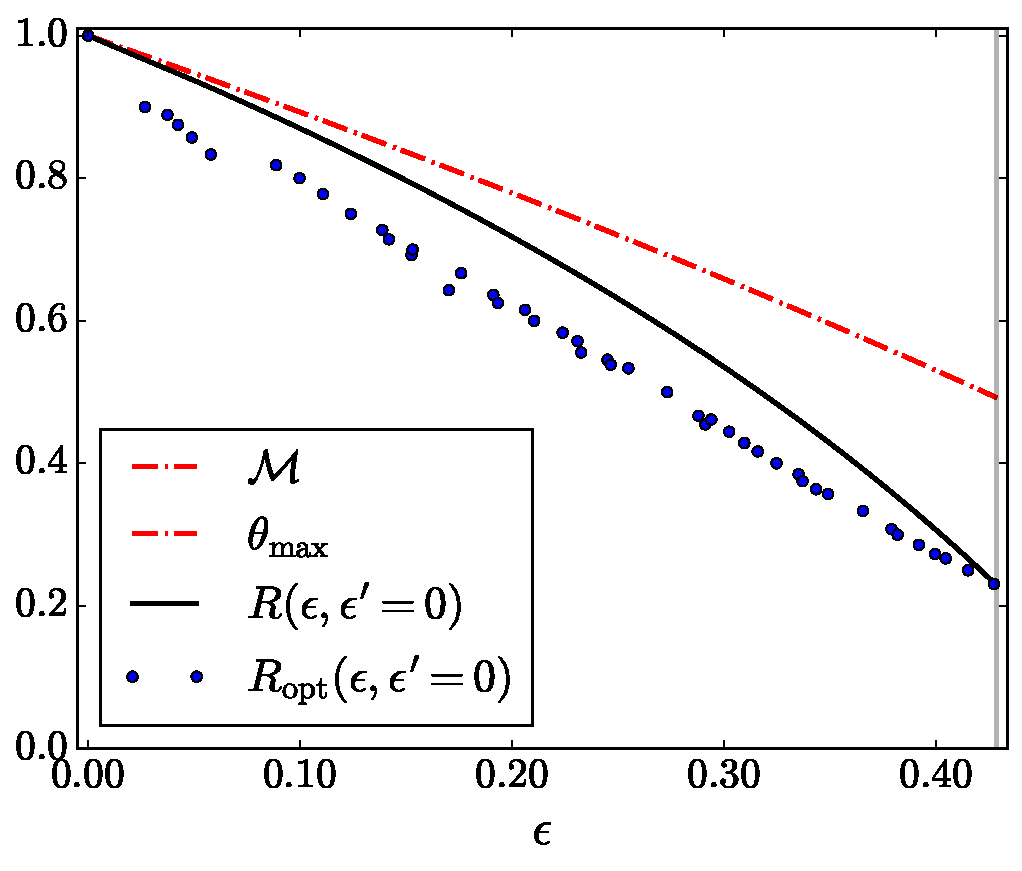
\includegraphics[scale=0.45]{figs/distill_bounds.pdf}
    \caption{\textbf{Distillation bounds in the unital fragment.} Distillation bounds obtained by the first elbow majorisation constraint $R$, mana $\M$ and max--thauma $\theta_{\rm{max}}$ are plotted for $\epsilon' = 0$, up to noise level $\epsilon = 3/7$.
    Majorisation provides stricter rates than the global mana and max--thauma bounds.
    Numerical bounds $R_{\rm{opt}}$ obtained by full Lorenz curve comparison for some Strange state purification processes with even number of copies $m,n \leq 30$ highlight that the first elbow constraint can be improved.
    }
    \label{fig:distill_bounds}
\end{figure}

In the next section we provide relative majorization bounds in arbitrary stabilizer fragments, and in particular we shall parameterize these bounds from a thermodynamic perspective. Specifically, we can interpret the stabilizer state $\sigma$, which defines the fragment, as a thermodynamic equilibrium state at some effective temperature and with some effective Hamiltonian.

\newpage
\section{Free energy dependent bounds for magic state distillation protocols}
\label{sec:stab}

We now consider a magic distillation protocol on multiple identical qudits in a noisy magic state $\rho(\epsilon)$, with noise parameter $\epsilon$, sending 
\begin{equation}
\rho(\epsilon)^{\otimes n} \longrightarrow \E(\rho(\epsilon)^{\otimes n}) =\rho(\epsilon')^{\otimes m}
\end{equation}
with $n \gg 1$ \nick{Should we replace $m$ with $R n$ throughout?}, $\epsilon' <\epsilon$ and $\E$ denoting the quantum channel induced by the protocol. We can now provide distillation bounds that depend on energetic and entropic aspects of the protocol. We do this relative to a reference temperature that can be chosen freely. The key idea is that the physical measures associated with this protocol are determined by how $\E$ would disturb a reference equilibrium state $\tau$ to some different state $\tau'$, if the protocol had been applied to this reference state instead of the $n$-copy magic state. 

More precisely, we assume each qudit has Hamiltonian $H$ and we choose some temperature $T = (k\beta)^{-1}$ where $k$ is Boltzmann's constant and $\beta$ the inverse temperature. The reference equilibrium state of the $n$ qudits is given by
\begin{equation}
\tau^{\otimes n} = \left ( \frac{e^{-\beta H}}{\Z} \right )  ^{\otimes n}.
\end{equation}
Since we are concerned with magic distillation we may assume that the reference state $\tau$ is not a magic state, so it has a non-negative Wigner distribution, and we shall further assume that it is a full-rank stabilizer state for the qudit. 

A given magic protocol on the $n$ qudits will correspond to a quantum channel $\E$. Our analysis associates to this protocol energy/entropy measures by considering how $\E$ transforms this reference equilibrium state. We first note that we can assume without loss of generality that $U_\pi\E(X) U_\pi^\dagger = \E(X)$ for all $X$ and any permutation $U_\pi$ of the $m$ output subsystems. This is justified because the protocol on the input magic state results in state $\rho(\epsilon')^{\otimes m}$, which is invariant under permutations. Therefore, we are always allowed to symmetrise the output $\E(X)$ by performing a group average over the permutation group for the output systems without changing the performance of the distillation protocol on $\rho(\epsilon)^{\otimes n}$. Thus, we can assume that $\E$ always outputs a symmetric state in general.

This means in particular that $\E(\tau^{\otimes n})$ is a symmetric state on $m$ subsystems, so by the quantum de Finetti theorem~\cite{christandl_2007} we have that
\begin{equation}
\E(\tau) \approx \int d\mu(x) \tau_x^{\prime \otimes m},
\end{equation}
where $d\mu(x)$ is a probability measure over a set $\{\tau'_x\}$ of single qudit states.

\subsection{Free energy measures and sub-linear correlations in the thermodynamic limit}
To simplify our analysis we will make the following assumption. We assume that in the asymptotic/thermodynamic limit $n,m \rightarrow \infty$ that correlations generated between subsystems are negligible. This implies that $d\mu(x)$ is peaked on a particular state $\tau'$, and so $\E(\tau) = \tau^{\prime \otimes m}$. Physically, this is a natural scenario -- for example, in the context of traditional thermodynamics, it states that the output system is well-described by intrinsic variables that are encoded in $\tau'$. Here, this assumption allows us to associate a free energy per qudit of the output state, which would be more complex if correlations are present.

The case of correlations between output subsystems can also be considered, but would lead to a more complex analysis within our majorization framework of Wigner distributions. In this direction, we highlight recent work in majorization in which stochastic independence and correlations are analysed. In particular, it has been shown that stochastic independence (no correlations) of independent distributions can be viewed as a resource in an extension of catalytic majorization, and leads to a single-shot operational interpretation of the Shannon entropy~\cite{muller_2015, muller_2016, muller_2019}.

Our analysis will depend on the energetic properties of the probe state $\tau$ and the output state $\tau'$.
For the state $\tau = e^{-\beta H}/\Z$, the Helmholtz free energy $F$ is given by
\begin{equation}
	F \coloneqq \tr[H \tau] - \beta^{-1}S(\tau) = -\beta^{-1}\log{\Z},
\end{equation}
which can be obtained from the internal energy via a Legendre transform~\cite{Pathria_1997}.

As mentioned, we can quantify the energetic aspects of a given protocol by considering how it transforms a physical system in state with a clear notion of energy, such as a thermodynamic equilibrium state. The protocol transforms this state as $\tau^{\otimes n} \rightarrow \E(\tau^{\otimes n}) = \tau^{\prime \otimes m}$.  Since the protocol does not, on its own, generate magic the output state $\tau'$ is also a stabilizer state, provided that $\tau$ is as well. This is generally a non-equilibrium state for the system. However, the distillation bounds that we derive take a particularly simple form if we associate a Hamiltonian $H'$ to the output state by considering the change $H \rightarrow H'$ such that equilibrium is restored at the reference temperature $T$. This Hamiltonian is defined by the expression $\tau' = e^{-\beta H'}/\Z'$, and has free energy $F' = -\beta^{-1} \log \Z'$.

\subsection{Free energy dependent bounds on magic state distillation protocols}
The preceding discussion gives a means to specify energetic details of a protocol through how much it would disturb some reference equilibrium state. When combined with relative majorization, it also allows us to derive magic distillation bounds that combine both the computational measures $\epsilon,\epsilon'$, with terms that depend on the Hamiltonian of the physical system. As discussed in section~\nick{REF}, from the perspective of majorization the presence of magic can be viewed as a form of non-classical free energy and so it is also of interest to make an explicit link between the amount of magic in a non-equilibrium state $\rho_S(\epsilon)$ and the actual free energy of an equilibrium state $\tau(\beta)$. 

Given this account we now state the following result for the case of $d=3$ qutrits, in which magic distillation protocols are viewed as non-equilibrium processes.

\begin{theorem}\label{thm:free-energy}
	Consider a magic distillation protocol on qutrits that transforms $n$ copies of an $\epsilon$--noisy Strange state into $m$ copies of an $\epsilon'$--noisy Strange state, with depolarising errors $\epsilon' \leq \epsilon \leq 3/7$. We also allow pre/post-processing by local Clifford unitaries.
	
	Let $T =(k\beta)^{-1}$ be any finite temperature for the physical system and let $H= \sum_{k \in \mathbb{Z}_3} E_k |E_k\>\<E_k|$ be the Hamiltonian of each qutrit subsystem in its eigen-decomposition.
Assume that in the thermodynamic limit ($n,m \gg 1$), the protocol applied to the equilibrium state $\tau^{\otimes n} = (e^{-\beta H}/\Z)^{\otimes n}$ maps $\tau^{\otimes n} \longrightarrow \tau^{\prime \otimes m}$, where we express state $\tau'$ as $\tau' = e^{-\beta H'}/\Z'$ for some Hermitian $H'$.

Then the magic distillation rate $R = m/n$ for the protocol is bounded by the expression
\begin{equation}\label{eq:rate_bounds_proof}
	R \leq \dfrac{\ln{\big( 1-\frac{4}{3}\epsilon \big)} + \beta (\phi - F)}{\ln{\big( 1-\frac{4}{3}\epsilon' \big)} + \beta (\phi' - F')},
\end{equation}
where $F$ is the free energy of $\tau$,  and 
\begin{equation}
	\phi = -\beta^{-1} \log \zeta
\end{equation}
with $\zeta$ given by the expressions
\begin{align}
	\zeta &= \sum_{k\in \mathbb{Z}_3} \alpha_k e^{-\beta E_k}, \nonumber\\
	\alpha_k &= \<E_k| A_{\x_\star} |E_k\>,
\end{align}
and $\x_\star = \arg\!\min W_\tau(\x)$. The primed variables are defined similarly for the output system.
\end{theorem}
\noindent The proof of this is provided in~\cref{free-energy-bound-proof}, and is a generalization of the analysis for unital protocols.

The above bound depends on: (a) quantum computational measures $\epsilon, \epsilon'$, (b) thermodynamic quantities $F, F',$  and (c) intermediate terms $\phi, \phi'$. The intermediate terms depend on how the energy eigenbasis of the system $\{|E_k\>\}$ relates to the computational stabilizer basis $\{|k\>\}$.  In particular, the energetic term $\phi$ quantifies the degree to which the negativity in the Wigner representation can be ascribed a sharp energetic value for the given Hamiltonian of the system. Its form is similar to $F$, and so can informally be viewed as a `magic free energy' term, associated to a `magic partition function' $\zeta$. The coefficients $\alpha_k$ may be negative for some $k$, when the Hamiltonian eigen-decomposes into non-stabilizer states, but the quantity $\phi$ is always well-defined, since the function $\zeta$ is a positive multiple of the stabilizer Wigner component $W_\tau(0,0)$, as seen in the proof of the theorem.

The sole purpose of the Clifford unitaries $C_1,C_2$ is to simplify the form of the $\alpha_k$ coefficients. \nick{That's not right, without Clifford processing we would get bounds that depend on $u$ whenever $\x_\star$ corresponds to $u$, as well as $v$ whenever $\x_\star$ corresponds to $v$ as seen in the contour plot - these are different values} For example, if $H=Z$ then the energy eigenbasis is equivalent to the computational basis up to a Fourier transform, and so $\phi$ would have a sharp, temperature-independent value $\phi \in \{E_0,E_1,E_2\}$ once we account for the Clifford change in basis. 

The above bound demonstrates how one can use relative majorization of quasi-distributions to incorporate additional information into distillation bounds.
The analysis involved makes simplifying assumptions that could easily be dropped, at the price of more complex expressions. For example, we can obtain general expressions without any assumptions on $\epsilon, \epsilon'$ or without performing any Clifford change in basis.
We could also perform similar analysis for general qudits, and different choices of magic states. It might also be of interest to consider other choices of reference states that may include more appropriate hardware physics, for example for photonic set-ups.

The only assumption that cannot be trivially dropped is the assumption that we can ignore correlations in the thermodynamic limit. This is a common situation in thermodynamics, where correlations are often sub-linear in the particle number in the macroscopic limit. One could perturb about this scenario, and make use of variational tools such as the Bogoliubov inequality~\cite{bogolyubov_1966} for approximating the free energy of a system, to obtain bounds in a similar form.

\begin{figure}[t!]
    \centering
    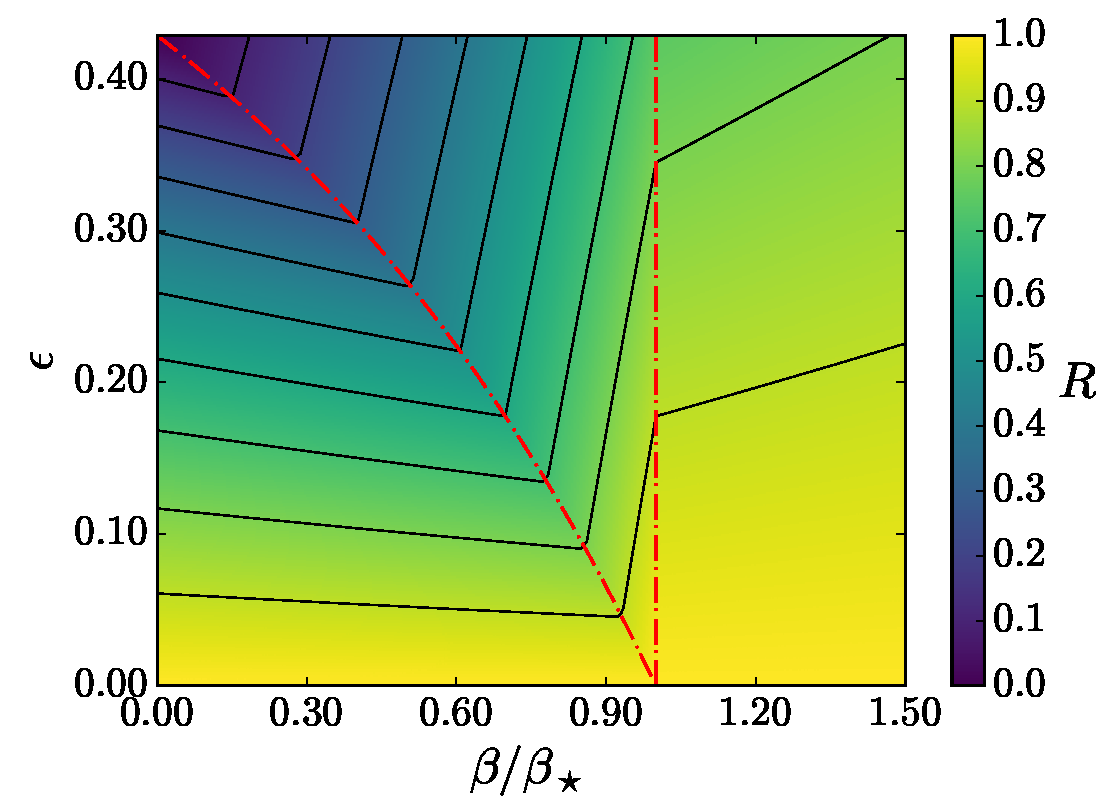
\includegraphics[scale=0.4]{figs/rate_scatter.pdf}
    \caption{\textbf{Temperature-dependent bounds for magic distillation.}
  Shown is a contour plot of the bound on $R(\epsilon, \beta)$ for $H = H' = \sum_{k \in \mathbb{Z}_3} k \ketbra{k}$ and $\epsilon' = 0$, where $\beta$ is the inverse temperature and $\epsilon$ the depolarising noise of the input magic state. The relevant data from the spectrum of the qutrit operator $H$ enters in via $\epsilon_\star(\beta)$ and $\beta_\star$. The vertical dashed line is the `Landauer-like' temperature threshold $\beta_\star$ and the diagonal dashed curve corresponds to the noise threshold $\epsilon_\star(\beta)$ for $\beta \leq \beta_\star$. \nick{Refer to definitions of starred quantities} The $\beta = 0$ line corresponds to the regime in which the magic protocol corresponds to a unital channel.
    }
    \label{fig:rate_contour}
\end{figure}

The bound derived is based on analysis of only part of the Lorenz curves and can be improved via a finer analysis.
This is apparent by simple numerical calculations on the entirety of the curves as seen in~\cref{fig:distill_bounds} for the case of unital operations.
Specifically, the existing bound follows by considering the dominant terms in the rescaled Wigner distribution and do not, for example, take into account the Lorenz curve's peak structure. 

As a special case of the result, suppose that $H=H'$, implying that the protocol leaves the equilibrium state unchanged, hence it corresponds to a Gibbs-preserving map~\cite{faist_2015}. We focus on the pure state distillation case, where $\epsilon' \rightarrow 0$, for which we obtain~\cref{fig:rate_contour}, a contour plot of the bound on $R$ as a function of inverse temperature $\beta$ and depolarising noise level $\epsilon$ for the initial noisy magic state.

In the more general case, $\Delta F \coloneqq F' - F \ne 0$ and we have a free energy difference between the initial and final states, with respect to the relevant Hamiltonians. This is similar to the free energy differences that occur in fluctuation relations, where the final state of the system can be arbitrarily far from equilibrium, yet a free energy term for the final system still arises.

\ddd{[Need some numerics on varying the $F'$ case]}

\section{Outlook and open questions}
\label{sec:lower_bounds}

\ddd{[Initial text. To be edited.]}
We have described how relative majorization can be used to establish upper bounds on magic distillation protocols that take into account additional physics of the system. Our bounds only exploited the very simplest aspects of the Lorenz curves of the quasi-distributions, so it would be of interest to sharpen these bounds and exploit more of the structure in the asymptotic limit. This raises interesting questions that do no arise for probability distributions, because we no longer have a notion of typicality and the central limit theorem does not apply. That said, for special states such as the Strange state the asymptotic behaviour is relatively simple, so one could study this and obtain a better handle on the asymptotic behaviour ($n \rightarrow \infty$). An example of such a question was raised regarding the numerical bounds plotted in~\cref{fig:distill_bounds} for the unital fragment. In~\cref{app:lcsu_technical} we give some more extensive analysis in the unital fragment that could be explored further, while in~\cref{app:lcst_technical} we also provide some tools which are useful in all fragments.

One might wonder if this approach could also provide \emph{lower bounds} for distillation protocols. Now, in contrast to the upper bounds, it is necessary to include the symplectic constraints on the phase space into the majorization relations.

For example, the Clifford group action on a quantum system corresponds to the action of the affine symplectic group~\cite{cit:gross3, cit:bengtsson} on the discrete phase space. Therefore, any convex mixture of Clifford unitaries will correpond to a convex mixture of these group actions. From the Hardy-Littlewood theorem~\cite{hardy_1952}, we know that traditional majorization is obtained from convex mixtures of arbitrary permutations. However, this has been generalised to convex mixtures of elements of a group $G$ that acts on vectors. This $G$--majorization has been studied in the classical literature and a range of results are known about it~\cite{giovagnoli_1985, steerneman_1990, eaton_1977}. For example, if $G$ is a finite reflection group then the $G$--majorization pre-order is described by a finite list of conditions~\cite{giovagnoli_1985}, just as is the case for the relative majorization ordering. One route leading to concrete lower bounds on distillation rates is therefore to consider reflection sub-groups of the affine symplectic, or just symplectic, group, for which the majorization relation reduces to a finite set of conditions.
  
The topic of $G$--majorization has been extensively studied, but to our knowledge there hasn't been work on relative $G$--majorization. This would correspond to transformations that are \emph{not} unital, but still respect the symplectic structure. Physically, this regime would correspond to a form of thermo-majorization obtained from looking at the action of the Clifford group at a micro-canonical level, and then reducing to a small subsystem~\cite{cit:lostaglio, Pathria_1997}. While this seems like a painful thing to consider, there is motivation for this beyond the aim of constructing lower bounds for magic protocols: in the case of statistical mechanics on a phase space this is precisely the situation, albeit in the continuum limit. Statistical mechanics of actual systems obey Hamiltonian dynamics and so automatically respect a symplectic form~\cite{Pathria_1997}. Therefore, the pre-order of statistical mechanical states with respect to phase space dynamics preserving a Gibbs state must correspond to a symplectic thermo-majorization condition. Of course, technical features arise in the continuum limit when considering distributions on an unbounded phase space, but this could be remedied by either considering a compact phase space (e.g. for a particle on a ring) or by first studying the discrete case. Such scenarios also arise in the Quantum Hall Effect~\cite{Klitzing_1980}, which is thus another regime where these techniques might be of use.

Finally, it would be of interest to consider the possibility of applying these techniques to other scenarios in which one wishes to distinguish classical from non-classical behaviour based on quasi-probability representations~\cite{Ferrie_2008, barnett_1997}

%%%%%%%%%%%%%%%%%%%%%%%%%%%%%%%%%%%%%%%%

\bibliography{bib}
%\bibliographystyle{apsrev4-2}

%%%%%%%%%%%%%%%%%%%%%%%%%%%%%%%%%%%%%%%%

\appendix
\newpage
\section{Properties of Wigner distributions}
\label{app:wigner}

Here, we present basic properties of the phase-point operators and the Wigner distribution that are used throughout the paper.

\begin{proposition}\label{thm:aproperties}
    For any dimension $d$, the phase-point operators satisfy:
    \begin{enumerate}
        \item[(i)]\label{en:a1} Hermiticity and unitarity: $A_{\bmx}^\dagger = A_{\bmx} = A_{\bmx}^{-1}$;
	    \item[(ii)]\label{en:a2} Closure under transposition: $A_{(x, p)}^T = A_{(x, -p)}$;
	    \item[(iii)]\label{en:a3} Unit trace for odd $d$: $\tr[A_{\bmx}] = 1$;
	    \item[(iv)]\label{en:a4} Completeness relation: $\sum_{\bmz \in \cal{P}_d} A_{\bmz} = d\id$;
	    \item[(i)]\label{en:a5} Orthogonality: $\tr[A_{\bmx}^\dagger A_{\bm{x'}}] = d \delta_{\bmx,\bm{x'}}$.
	\end{enumerate}
\end{proposition}
All properties follow from the definition in~\cref{eq:ax} along with properties of the displacement operator $D_{\bmx}$ and can be found in the literature, e.g.~\cite{cit:veitch,Vourdas_2004,cit:gross3}

\begin{proposition}\label{thm:wstate}
  The Wigner distribution of a state $\rho \in \cal{B}(\cal{H}_d)$ is
  \begin{enumerate}
    \item[(i)]\label{en:w1} Real valued: $\W{\rho} \in \mathbb{R}^{d^2}$;
    \item[(ii)]\label{en:w2} Normalised: $\sum_{\bmz \in \cal{P}_d} \W[\bmz]{\rho}=1$;
    \item[(iii)]\label{en:w3} Bounded: $\abs{\W[\bmx]{\rho}} \leq \frac{1}{d}$.
    \item[(iv)]\label{en:w4} Additive under mixing: \vspace{2pt}\\
    $\W[\bmx]{p\rho_1 + (1-p)\rho_2} = p\W[\bmx]{\rho_1} + (1-p)\W[\bmx]{\rho_2}$;
    \item[(v)]\label{en:w5} Multiplicative under tensor products: \vspace{2pt}\\
    $\W[\bmx_A \oplus \bmx_B]{\rho_A \otimes \rho_B} = \W[\bmx_A]{\rho_A}\W[\bmx_B]{\rho_B}$.
	\end{enumerate}
\end{proposition}
\begin{proof}
	Proof of all properties can be found in the literature~\cite{cit:veitch,Vourdas_2004,cit:gross3,Wang_2019} except for property (iii) which we prove here.
	
Let $\{\lambda_i\}_{i \in \mathbb{Z}_d}$ be the (non-negative) eigenvalues of $\rho$, summing to 1.
Let $\{\alpha_{\bmx,i}\}_{i \in \mathbb{Z}_d}$ be the eigenvalues of $A_{\bmx}$. For any $\bmx, \alpha_{\bmx,i} \in \{-1, 1\}$, due to the hermiticity and unitarity of the phase-point operators. 
Then,
\begin{align}
	\abs{W_{\rho}(\bmx)} &= \frac{1}{d}\abs{\tr[A_{\bmx} \rho]} \leq \frac{1}{d} \abs{\sum_i \alpha_{\bmx,i} \lambda_i} \nonumber\\ &\leq \frac{1}{d}\sum_i \lambda_i = \frac{1}{d}.
\end{align}
The first inequality follows from Theorem 1 of~\cite{cit:mirsky} for the trace of complex matrices, while the second is the Cauchy-Schwarz inequality.
\end{proof}

\begin{proposition}
    \label{thm:wchannel}
    The Wigner distribution of a $\cptp$ operation $\E: \cal{B}(\cal{H}_{d_A}) \mapsto \cal{B}(\cal{H}_{d_B})$ is
    \begin{enumerate}
        \item[(i)]\label{en:wo1} Real-valued: $\W{\E} \in \mathbb{R}^{d^2} \times \mathbb{R}^{d^2}$;
        \item[(ii)]\label{en:wo2} Normalised: $\sum_{\bmz \in \cal{P}_{d_B}} \W[\bmz|\bmx]{\E} = 1$ \\ 
        for any $\bmx \in \cal{P}_{d_A}$;
        \item[(iii)]\label{en:wo3} Bounded: $\abs{\W[\bmy|\bmx]{\E}} \leq \frac{d_A}{d_B}$;
	    \item[(iv)]\label{en:wo4} Transitive: $\W[\bmy]{\E(\rho)} = \sum_{\bmz \in \cal{P}_{d_A}} \W[\bmy|\bmz]{\E} \W[\bmz]{\rho}$ for any $\bmy \in \cal{P}_{d_B}$.
    \end{enumerate}
\end{proposition}
If $d_A = d_B$, and in particular if operation $\E$ maps a Hilbert space onto itself, then the stochasticity condition $\abs{\W[\bmy|\bmx]{\E}} \leq 1$ is satisfied.
\begin{proof}
	Proof of all properties are provided by Wang \textit{et al.}~\cite{Wang_2019} except for property (iii) which is a direct consequence of the definition of $\W{\E}$ and the corresponding property (iii) in~\cref{thm:wstate}.
\end{proof}

%%%%%%%%%%%%%%%%%%%%%%%%%%%%%%%%%%%%%%%%

\section{Properties of majorization}
\label{app:major}
	
We now give the following equivalent formulations of $d$--majorization.

\begin{proposition}\label{prop:rmajor}
Given $\bmx, \bmy, \r \in \mathbb{R}^n$, such that the components of $\r$ are positive, the following statements are equivalent:
  \begin{enumerate}
    \item[(i)] $\bmy = A\bmx$ and $\r = A\r$ for a stochastic map $A$;
    \item[(ii)]\label{en:tm3} $\sum\limits_{i=1}^n \abs{x_i - r_i t} \leq \sum\limits_{i=1}^n \abs{y_i - r_i t}$ for all $t \in \mathbb{R}$;
    \item[(iii)] $L_{\bmx|\r}(t) \leq L_{\bmy|\r}(t)$ for $t\in [0,1)$ and \vspace{5pt}\\ $L_{\bmx|\r}(1) = L_{\bmy|\r}(1)$.
  \end{enumerate}
\end{proposition}
The proofs for these can be found in~\cite{cit:marshall,cit:bhatia,cit:nielsen,cit:lostaglio} and references therein.

The following result is used in the text to relate relative majorization of quasi-distributions to their Lorenz curves.
\begin{proposition}\label{lemma:Lorenz_linearity}
	Let $\p$ be a quasi-probability distribution and let $\r$ be a probability distribution with strictly non-zero components. Let $a > 0$ and $b \in \mathbb{R}$ then $L_{a\p + b \r | \r} (x) = a L_{\p |\r}(x) + b x$.
\end{proposition}
\begin{proof} 
	The Lorenz curve of $a\p + b \r$ relative to $\r$ passes through $(0,0)$ and the points $(\sum_{i=1}^k{r_{\pi(i)}}, \sum_{i=1}^k(a \p + b \r)_{\pi(i)})$ where $\pi$ is the permutation that puts $(a p_i/r_i + b)$ in non-increasing order. Since $a > 0$, the permutation $\pi$ puts  $(p_i/r_i)$ in non-increasing order too. We thus have
\begin{align*}
&\left( \sum_{i=1}^kr_{\pi(i)}, \sum_{i=1}^k(a \p + b \r)_{\pi(i)} \right) = \\ 
&\left( \sum_{i=1}^k r_{\pi(i)},a \sum_{i=1}^k  p_{\pi(i)} + b\sum_{i=1}^k r_{\pi(i)} \right) \nonumber,
\end{align*}
so the value of the Lorenz curve at each potential elbow point $x_k = \sum_{i=1} ^kr_{\pi(i)}$ is given by
\begin{align}
&L_{a \p +b \r|\r} (x_k) = a L_{\p|\r} (x_k) + b L_{\r|\r}(x_k) = \nonumber\\
&a L_{\p|\r} (x_k) + b x_k,
\end{align}
so we have $L_{a\p  + b\r|\r} (x) = a L_{\p |\r}(x) + b x$ for any $x \in [0,1]$ due to linearity.
\end{proof}

\begin{theorem*}
	Given a magic state $\rho$, the maximum $L_\star$ of its Lorenz curve $\lc{\rho}{\sigma}(x)$ is independent of the $\sigma$--fragment and equal to $1+\sn{\rho}$. Moreover, the majorization constraint is stronger than mana in every fragment.
\end{theorem*}
\begin{proof}
	We denote the Wigner distributions of the states compactly as vectors $\bmw(\rho) \equiv W_\rho(x)$ and $\bmw(\sigma) \equiv W_\sigma(x)$.
	We choose the component indexing so that the rescaled distribution 
	\begin{equation}
		\widetilde{\bmw}(\rho|\sigma) \coloneqq \left(\frac{w(\rho)_1}{w(\sigma)_1}, \dots, \frac{w(\rho)_{d^2}}{w(\sigma)_{d^2}} \right)^T,
	\end{equation}
	is sorted, $\widetilde{\bmw} = \widetilde{\bmw}^\downarrow$.
	Note that all components of $\bmw(\sigma)$ are positive, so $\widetilde{w}_i \geq 0$ if and only if $w(\rho)_i \geq 0$ for any $i=1,\dots,d^2$.
	
	Let $i_\star$ be the index of the smallest non-negative component of $\widetilde{\bmw}^\downarrow$.
	Then, $w(\rho)_i < 0$ if and only if $i > i_\star$, so the maximum of Lorenz curve $\lc{\rho}{\sigma}(x)$ takes the value 
	\begin{equation}
		\lc{\rho}{\sigma}(x_{i_\star}) = \sum_{i=1}^{i_\star} w(\rho)_i,
	\end{equation}
	and is achieved at
	\begin{equation}\label{eq:maxloc}
		x_{i_\star} \coloneqq \sum_{i=1}^{i_\star} w(\sigma)_i.
	\end{equation}

	The location of the maximum ($x=x_{i_\star}$) varies from fragment to fragment, but its value is independent of $\sigma$,
	\begin{align}
	L_\star &:=	\lc{\rho}{\sigma}(x_{i_\star}) 
		= \sum\limits_{\bmx: \W[\bmx]{\rho} \geq 0} \W[\bmx]{\rho} \nonumber \\
		&= 1 + \sn{\rho}.
	\end{align}
	
Since the magic monotone mana is a monotonic function of sum-negativity, $\rm{mana}(\rho) \coloneqq \ln{(2\hspace{1pt}\sn{\rho}+1)}$, we see that mana corresponds precisely to the peak of the Lorenz curve $L_{\rho|\sigma}(x)$. Therefore, mana is one of $d^{2n}$ constraints, so majorization is strictly a stronger constraint in any fragment.
\end{proof}



%%%%%%%%%%%%%%%%%%%%%%%%%%%%%%%%%%%%%%%%

\section{Technical properties of $\sigma$--fragments}
\label{app:frag}

In this section, we discuss some technical aspects of general $\sigma$--fragments.

We first prove a result on the independence of the Lorenz curve constraints, stated in~\cref{sec:major_frag}.
\begin{proposition}\label{thm:elbows}
	Let $\rho, \tau$ be two quantum states with Lorenz curves $\lc{\rho}{\sigma}(x), \lc{\tau}{\sigma}(x)$ in the $\sigma$--fragment.
	
	Let $t$ be the number of elbows of $\lc{\tau}{\sigma}(x)$ at locations $x_1, \dots, x_t$.
	
	Then, $\lc{\rho}{\sigma}(x) \geq \lc{\tau}{\sigma}(x)$ for all $x \in [0,1]$ iff $\lc{\rho}{\sigma}(x_{i}) \geq \lc{\tau}{\sigma}(x_{i})$ for all $i =1,\dots,t$.
\end{proposition}
\begin{proof}	
	$\lc{\rho}{\sigma}(x) \geq \lc{\tau}{\sigma}(x)$ for all $x \in [0,1]$ trivially implies $\lc{\rho}{\sigma}(x_{i}) \geq \lc{\tau}{\sigma}(x_{i})$ for all $i = 1,\dots,n'$.
	
	Conversely, assume that $\lc{\rho}{\sigma}(x_{i}) \geq \lc{\tau}{\sigma}(x_{i})$ for all $i = 1,\dots,r$.
	First, let $x_0 = 0$ and $x_{n'+1} = 1$, so that $\lc{\rho}{\sigma}(x_0) = \lc{\tau}{\sigma}(x_0) = 0$ and $\lc{\rho}{\sigma}(x_{n'+1}) = \lc{\tau}{\sigma}(x_{n'+1}) = 1$.
	Hence, we can extend the set of elbows $E$ to $E' = E \cup \{x_0, x_{n'+1}\}$.
	
	Pick two consecutive locations $x_{i}, x_{i+1}$ in $E'$ and consider the line segment $\ell_\tau(x)$ connecting points $(x_{i}, \lc{\tau}{\sigma}(x_{i}))$ and $(x_{i+1}, \lc{\tau}{\sigma}(x_{i+1}))$ as well as the line segment $\ell_\rho(x)$ connecting points $(x_{i}, \lc{\rho}{\sigma}(x_{i}))$ and $(x_{i+1}, \lc{\rho}{\sigma}(x_{i+1}))$.
	This is illustrated in~\cref{fig:elbows_proof}.
\begin{figure}[h]
    \centering
    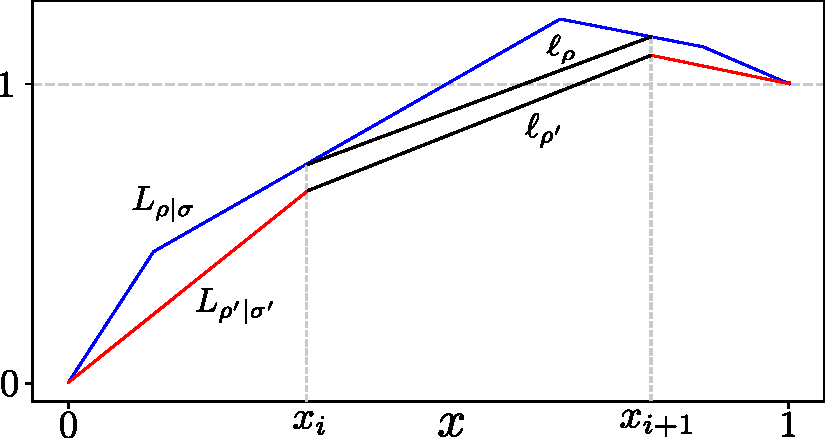
\includegraphics[scale=0.5]{figs/elbows_proof.pdf}
    \caption{\textbf{Illustration of~\cref{thm:elbows}}.
    }
    \label{fig:elbows_proof}
\end{figure}

	Due to concavity of $\lc{\rho}{\sigma}$, it is clear that for all $x \in [x_{i}, x_{i+1}]$, we have $\lc{\rho}{\sigma}(x) \geq \ell_\rho(x) \geq \ell_\tau(x) = \lc{\tau}{\sigma}(x)$.
	This argument can be made in all intervals $[x_{i}, x_{i+1}]$ with $i=0,\dots,n'$, so the proof is complete.
\end{proof}
The above theorem can be of practical importance in reducing the necessary distillation constraints derived via majorization in $\sigma$--fragments.

\begin{proposition}\label{thm:frag_app}
    Let $\R = (\F, \O)$ be a magic theory and $\sigma, \sigma' \in \F$. The following statements hold:
    \begin{enumerate}
        \item No $\sigma$--fragment of $\R$ is empty.
        \item If a free operation leaves two states invariant, then it also leaves their mixtures invariant, 
        \begin{equation*}
            \O_{\sigma} \cap \O_{\sigma'} \subseteq \O_{p\sigma + (1-p)\sigma'}\ \text{for any}\ p \in [0,1].
        \end{equation*}
    \end{enumerate}
\end{proposition}
\begin{proof}$ $\vspace{-12pt}\\

\begin{enumerate}
    \item The identity channel $1_{\rm{C}}$ belongs to every $\sigma$--fragment, as $1_{\rm{C}} \in \O$ and $1_{\rm{C}}\sigma = \sigma$ for all $\sigma \in \F$.
    
    \item Let $\E \in \O_{\sigma} \cap \O_{\sigma'}$.
    Then $\E \in \cptp$ and corresponds to stochastic Wigner distribution $\W{\E}$ such that $\W{\E} \W{\sigma} = \W{\sigma}$ and $\W{\E} \W{\sigma'} = \W{\sigma'}$.
    Then, $\W{\E} \W{p\sigma + (1-p)\sigma'} = \W{p\sigma + (1-p)\sigma'}$ for any $p \in [0,1]$ due to the additive property~\ref{en:w4} of the Wigner distribution, implying that state $p\sigma + (1-p)\sigma'$ is also left invariant by $\E$.
\end{enumerate}
\vspace{-20pt}
\end{proof}

Any free state $\sigma \in \F$ corresponds to a $d^2$--dimensional probability distribution $\W{\sigma}$ and any free operation $\E \in \O$ corresponds to a $d^2 \times d^2$ stochastic matrix (or conditional probability distribution) $\W{\E}$.
Note that these mappings are one-to-one due to the orthogonality of the phase-point operators as an operator basis.
Note further that free states $\F$ are mapped onto a \emph{strict subset} of the set of probability distributions.
As a counterexample, the sharp $d^2$--dimensional probability distribution $(1, 0, \dots, 0)$ does not correspond to any qudit Wigner distribution because of the boundedness condition in~\cref{thm:wstate}.
Similarly, not all stochastic matrices correspond to completely positive operations.
As an example, consider the permutation matrix
\begin{equation}
    \Pi_X = \begin{psmallmatrix}
        0 & 1 & 0 & 0 & 0 \\
        0 & 0 & 0 & 0 & 1 \\
        0 & 0 & 0 & 1 & 0 \\
        1 & 0 & 0 & 0 & 0 \\
        0 & 0 & 1 & 0 & 0
    \end{psmallmatrix} \otimes \begin{psmallmatrix}
        0 & 0 & 1 & 0 & 0 \\
        0 & 0 & 0 & 0 & 1 \\
        0 & 0 & 0 & 1 & 0 \\
        1 & 0 & 0 & 0 & 0 \\
        0 & 1 & 0 & 0 & 0    
    \end{psmallmatrix} \in {\rm{S}}_5({\W{\frac{1}{5}\id}}).
\end{equation}
It preserves the uniform distribution $\W{\frac{1}{5}\id}$, but it does not correspond to any positive (hence quantum) operation.

%%%%%%%%%%%%%%%%%%%%%%%%%%%%%%%%%%%%%%%%

\section{Lorenz curves in the unital fragment}
\label{app:lcsu_technical}

\subsection{Binomial distributions and error bounds}\label{app:phi}
Consider an experiment consisting of $n$ trials of throwing a $p$--coin, that is a coin with probability $p$ of landing on one side and $1-p$ of landing on the other.
We express the sums over an even number $m$ of successful trials $\Phi_+$ and an odd number $m$ of successful trials $\Phi_-$,
\begin{align}	
	\Phi_+(m; n, p) &\coloneqq \sum\limits_{\ell=0}^{m/2} \binom{n}{2\ell} p^{2\ell} (1-p)^{n-2\ell}, \nonumber\\ 
	&\text{for even integers } m\in[0,n], \label{eq:fp_app} \\
	\Phi_-(m; n, p) &\coloneqq \sum\limits_{\ell=1}^{(m-1)/2} \binom{n}{2\ell+1} p^{2\ell+1} (1-p)^{n-(2\ell+1)}, \nonumber\\ 
	&\text{for odd integers }m\in[0,n]. \label{eq:fn_app}
\end{align}
Note that index $m$ only takes even (odd) values when labelling $\Phi_+$ ($\Phi_-$).
In~\cref{app:lcsu_coord}, we will use $\Phi_+$ and $\Phi_-$ to express the elbow coordinates of Lorenz curves in the unital fragment.

We also define the classical entropy of a $p$--coin and the classical relative entropy between a $p$--coin and a $q$--coin,
\begin{align}
	S(p) &\coloneqq -p\log{p} -(1-p)\log{(1-p)}, \label{eq:ent}\\
	\ent{p}{q} &\coloneqq p \log{\frac{p}{q}} + (1-p) \log{\frac{1-p}{1-q}}. \label{eq:ent_rel}
\end{align}
They are symmetric in the sense that $S(p) = S(1-p)$ and $\ent{p}{q} = \ent{1-p}{1-q}$.

A useful result is the entropic bound on a combination~\cite{cit:ash}.
\begin{lemma}\label{lem:comb_bounds}
	For all $\ell\in [1,n-1]$,
	\begin{align}
		&\left[ 8\ell\left(1-\frac{\ell}{n}\right) \right]^{-\frac{1}{2}} 2^{n S\left(\frac{\ell}{n}\right)} \leq \binom{n}{\ell} \leq \\
		&\left[ 2\pi \ell\left(1-\frac{\ell}{n}\right) \right]^{-\frac{1}{2}} 2^{n S\left(\frac{\ell}{n}\right)}.
	\end{align}
\end{lemma}
The proof provided in~\cite{cit:ash} proceeds with direct calculation for the edge cases $\ell = 1,2, n-1, n-2$ and use Stirling's approximation for the remaining cases.
We can use~\cref{lem:comb_bounds} to provide strict upper and lower bounds on the functions $\Phi_+, \Phi_-$.

\subsection{Theory on bounding the core functions}
\nick{Should we really keep this section? It is standard calculus and the bounds are really loose.}
Here we present a more manageable method of bounding the core functions $\Phi_{\pm}$, which however results in looser bounds. 
We can rewrite the functions as
\begin{equation}
	\Phi_{\pm}(m; n, a) = \frac{1}{2}(\Phi(m; n, a) \pm (1+a)^{-n} S(m; n, a)),
\end{equation}
where we have substituted $a = p/(1-p)$. 
$\Phi$ is the standard cumulative function
\begin{equation}
	\Phi(m; n, a) = (1+a)^{-n} \sum_{k=0}^m \binom{n}{k} a^k,
\end{equation}
and the remainder term is
\begin{equation}
	S(m; n, a) \coloneqq \sum_{k=0}^m \binom{n}{k} (-a)^k.
\end{equation}
We have the following asymptotic bounds on the behaviour of $\Phi$~\cite{cit:ash},
\begin{lemma}\label{lem:phi_bounds}
	Given fixed $n>0$ and $p$, $\Phi$ satisfies the following bounds:
	\begin{align*}
		\begin{split}
		&\text{1. } \Phi(m; n, p) \geq \left[ 8m\left(1-\frac{m}{n}\right) \right]^{-\frac{1}{2}} 2^{-n\ent{\frac{m}{n}}{p}}, \\
		&\hspace{14pt} m\in [1,n-1] \\
		&\text{2. } \Phi(m; n, p) \geq 1 - 2^{-n\ent{\frac{m+1}{n}}{p}},\ m\in [np+1,n-2] \\
		&\text{3. } \Phi(m; n, p) \leq 1 - \left[ 8(m+1)\left(1-\frac{m+1}{n}\right) \right]^{-\frac{1}{2}}\times \\
		&\hspace{14pt} 2^{-n\ent{\frac{m+1}{n}}{p}},\ m\in [0,n-2]
		\end{split}
		\\
		&\text{4. } \Phi(m; n, p) \leq 2^{-n\ent{\frac{m}{n}}{p}},\ m\in [0,np]
	\end{align*}
\end{lemma}

We would like some theory that estimates the value of $S(m; n, a)$ for different parameter regimes. 
We can consider the function $f(x) = (1+x)^n$ and note that $S(m; n, a)$ is the $m$'th partial sum of this expansion at the point $x=-a$.

The truncated Maclaurin series of a general function $f(x)$ is
\begin{equation}
	f(x) = f(0) + x f'(0) + \dots \frac{x^m}{m!}f^{(m)}(0) + R_m(x)
\end{equation}
with a remainder term
\begin{align}
	R_m (x)&= \int_{0}^x dt f^{(m+1)}(t) \frac{(x-t)^m}{m!} \\
	&= \frac{x^{m+1}}{(m+1)!} f^{(m+1)}(x_*),
\end{align}
where in the second expression, $x_*$ is an implicit point that lies between $0$ and $x$ that comes from the Mean Value Theorem.

Applying this to the function $f(x) = (1+x)^n$ gives
\begin{equation}
	(1+x)^n = \sum_{k=0}^m \binom{n}{k} x^k + R_m.
\end{equation}
Evaluating at $x=-a$ gives
\begin{equation}
	S(m; n, a) = (1-a)^n - R_m(-a),
\end{equation}
where the key remainder term is given by
\begin{align}
	R_m(-a) &= \int_0^{-a} dt f^{(m+1)}(t) \frac{(-a-t)^m}{m!} \\
&= \frac{(-a)^{m+1}}{(m+1)!} f^{(m+1)}(x_*).
\end{align}
We can also compute the derivative $f^{(m+1)}(x)$ explicitly,
\begin{equation}
	f^{(m+1)}(x) = (m+1)!\binom{n}{m+1}(1+x)^{n-m-1}.
\end{equation}
Therefore, we have that
\begin{align}
	R_m(-a) &= (-1)^{m+1}(m+1)\binom{n}{m+1}\times \nonumber\\
	&\hspace{12pt} \int_{-a}^0 dt (1+t)^{n-m-1}(a+t)^m \\
&= \binom{n}{m+1}(-a)^{m+1}(1+x_*)^{n-m-1},
\end{align}
where in the latter expression $x_* \in [-a,0]$. 
Note that the first integral expression can be estimated via the Cauchy-Schwarz or the H{\"o}lder inequality. 
Therefore, we can either work with an explicit form with an unknown (but bounded) parameter $x_*$, or we can use the integral form and provide concrete estimates on it value.

A very simple estimate, based on $x_*$ lying in the interval $[-a,0]$ gives
\begin{equation}
(1-a)^{n-m-1} \leq \frac{R_m(-a)}{\binom{n}{m+1}(-a)^{m+1}} \leq 1,
\end{equation}
which in turn leads to the following bounds on $\Phi_+(m; n, a)$:
\begin{align}
	\hspace{-2cm}2\Phi_+(m; n, a) \leq\ &\Phi(m; n, a) + (1-a)^n - \frac{(-a)^{m+1}}{m!} \times \nonumber\\
	 &\binom{n}{m+1} (1-a)^{n-m-1} \text{ and} \\
	2\Phi_+(m; n, a) \geq\ &\Phi(m; n, a) + (1-a)^n - \frac{(-a)^{m+1}}{m!} \binom{n}{m+1} .
\end{align}

\subsection{Lorenz curve coordinates in the unital fragment}\label{app:lcsu_coord}
The Wigner distribution of the $n$--copy qutrit maximally mixed state $\left(\id/3\right)^{\otimes n}$ is the uniform probability distribution over the phase space, consisting of $9^n$ components equal to $9^{-n}$.
The Wigner distribution of the 1-copy $\epsilon$--noisy Strange state $\rho_{\rm{S}}(\epsilon)$ in the unital fragment consists of some permutation of a single negative component
\begin{equation}
	- v(\epsilon) \coloneqq - \left( \frac{1}{3} -\frac{4}{9}\epsilon \right),
\end{equation} 
and $8$ positive components
\begin{equation}
	u(\epsilon) \coloneqq \frac{1}{6} -\frac{1}{18}\epsilon.
\end{equation}
where in the unital fragment we need the condition $0 \leq \epsilon < 3/4$, so that the state contains some Wigner negativity ($-v < 0$).
It is also clear that $v \geq u$ in the interval $0 \leq \epsilon \leq 3/7$, while $u > v$ in the interval $3/7 < \epsilon < 3/4$.

The Wigner distribution of the $n$--copy $\epsilon$--noisy Strange state $\rho_{\rm{S}}(\epsilon)^{\otimes n}$ in the unital fragment is given by the convolution $\W{\rho_{\rm{S}}(\epsilon)^{\otimes n}} = W_{\rho_{\rm{S}}(\epsilon)}^{\otimes n}$.
In general, $\rho_{\rm{S}}(\epsilon)^{\otimes n}$ contains $n + 1$ distinct components, labelled $0,\dots, n$.
We present the distinct Wigner components of $\rho_{\rm{S}}(\epsilon)^{\otimes n}$ along with their multiplicites in~\cref{tab:lcsu}.
Note that LHS (RHS) refers to elbow coordinates $i$ on the left of and including (right of) the Lorenz curve maximum, stated precisely as
\begin{align}
&\text{LHS: } 0 \leq i \leq \left\lfloor \frac{n}{2} \right\rfloor \text{ and} \\
&\text{RHS: } \left\lfloor \frac{n}{2} \right\rfloor +1 \leq i \leq n.
\end{align}
\begin{table}[h]
  \def\arraystretch{1.5}
  \centering
  \begin{tabular}{c|c|c|r|r}
    \multicolumn{3}{c|}{Case} & \multicolumn{1}{c}{$m_{i}(n, \epsilon)$} & \multicolumn{1}{|c}{$w_{i}(n, \epsilon)$} \\[0.5ex]\hline
    \multirow{4}{*}{\raisebox{-4ex}{\rotatebox[origin=c]{90}{$0\leq \epsilon < \frac{3}{7}$}}} & \hspace{0.8ex}\multirow{2}{*}{\raisebox{-1ex}{\rotatebox[origin=c]{90}{$n$ even}}}\hspace{0.8ex} & LHS & $8^{2i}\binom{n}{2i}$ & $\left( \frac{1}{6} - \frac{1}{18}\epsilon \right)^{2i}\left( -\frac{1}{3} + \frac{4}{9}\epsilon \right)^{n-2i}$ \\
    & & RHS & $8^{n-2i}\binom{n}{2i}$ & $\left( \frac{1}{6} - \frac{1}{18}\epsilon \right)^{n-2i}\left( -\frac{1}{3} + \frac{4}{9}\epsilon \right)^{2i}$ \\ \cline{2-5}
    & \multirow{2}{*}{\raisebox{-2ex}{\rotatebox[origin=c]{90}{$n$ odd}}} & LHS & $8^{2i+1}\binom{n}{2i+1}$ & $\left( \frac{1}{6} - \frac{1}{18}\epsilon \right)^{2i+1}\left( -\frac{1}{3} + \frac{4}{9}\epsilon \right)^{n-2i-1}$ \\
    & & RHS & $8^{n-2i-1}\binom{n}{2i+1}$ & $\left( \frac{1}{6} - \frac{1}{18}\epsilon \right)^{n-2i-1}\left( -\frac{1}{3} + \frac{4}{9}\epsilon \right)^{2i+1}$ \\ \hline
    \multirow{4}{*}{\raisebox{-4ex}{\rotatebox[origin=c]{90}{$\frac{3}{7}\leq \epsilon < \frac{3}{4}$}}} & \multirow{2}{*}{\raisebox{-1ex}{\rotatebox[origin=c]{90}{$n$ even}}} & LHS & $8^{n-2i}\binom{n}{2i}$ & $\left( \frac{1}{6} - \frac{1}{18}\epsilon \right)^{n-2i}\left( -\frac{1}{3} + \frac{4}{9}\epsilon \right)^{2i}$ \\
    & & RHS & $8^{2i}\binom{n}{2i}$ & $\left( \frac{1}{6} - \frac{1}{18}\epsilon \right)^{2i}\left( -\frac{1}{3} + \frac{4}{9}\epsilon \right)^{n-2i}$ \\ \cline{2-5}
    & \multirow{2}{*}{\raisebox{-2ex}{\rotatebox[origin=c]{90}{$n$ odd}}} & LHS & $8^{n-2i}\binom{n}{2i}$ & $\left( \frac{1}{6} - \frac{1}{18}\epsilon \right)^{n-2i}\left( -\frac{1}{3} + \frac{4}{9}\epsilon \right)^{2i}$ \\
    & & RHS & $8^{2i}\binom{n}{2i}$ & $\left( \frac{1}{6} - \frac{1}{18}\epsilon \right)^{2i}\left( -\frac{1}{3} + \frac{4}{9}\epsilon \right)^{n-2i}$ \\ \hline
  \end{tabular}
  \caption{Wigner components $w_{i}(n, \epsilon)$ of $\rho_{\rm{S}}(\epsilon)^{\otimes n}$ along with their multiplicities $m_{i}(n, \epsilon)$, with $0 \leq i \leq n$.
  The expressions change depending on the noise level $\epsilon$, the parity of the number of copies $n$ and whether the index $i$ is lower or higher than the index of the Lorenz curve maximum (LHS vs RHS).
  Multiplication $2i$ is considered modulo $(n+1)$.}
  \label{tab:lcsu}
\end{table}

Every Lorenz curve in the unital fragment contains $n$ elbows, which, along with the boundary points $(x_{-1}, L_{-1}) = (0,0)$ and $(x_{n}, L_{n}) = (1,1)$, are labelled by 
\begin{equation*}
\{(x_{i}, L_{i})\}_{i=-1,0,\dots,n}.
\end{equation*}
The maximum is the $\lfloor n/2 \rfloor$-th elbow and its coordinates are calculated by collecting all the positive Wigner components,
\begin{align}
	x_{\lfloor n/2 \rfloor} &= \frac{1}{2}\left(1 + \left(\frac{7}{9}\right)^n\right), \\
	L_{\lfloor n/2 \rfloor} &= \frac{1}{2}\left (1 + \left(\frac{15 - 8\epsilon}{9}\right)^n \right).
\end{align}
%\sum_{j: even}^n a^j \binom{n}{j} = \frac{1}{2} [ (1+a)^n + (1-a)^n ]

Expressions for all the elbow coordinates follow from summing up the Wigner components in decreasing order.
In~\cref{tab:lcsu_coord_elb_app}, we present the elbow coordinates of the $n$-copy, $\epsilon$--noisy Strange state Lorenz curve in the unital fragment for any combination of parameters $n, \epsilon$.
\begin{table}[h]
  \def\arraystretch{1.5}
  \centering
  \begin{tabular}{c|c|c|r|r}
\multicolumn{3}{c|}{\multirow{2}{*}{Case}} & \multicolumn{1}{c|}{$x_{i}$} & \multicolumn{1}{c}{$L_{i}$} \\
    \multicolumn{3}{c|}{} & \multicolumn{1}{c|}{$x_{i} - x_{\lfloor n/2 \rfloor}$} & \multicolumn{1}{c}{$L_{i} - L_{\lfloor n/2 \rfloor}$} \\[0.5ex]\hline 
    \multirow{4}{*}{\raisebox{-5ex}{\rotatebox[origin=c]{90}{$0\leq \epsilon < \frac{3}{7}$}}} & \hspace{0.8ex}\multirow{2}{*}{\raisebox{-3ex}{\rotatebox[origin=c]{90}{$n$ even}}}\hspace{0.8ex} & LHS & $\Phi_+\left(2i;n,\frac{8}{9}\right)$ & $\left( \frac{5}{3} - \frac{8}{9}\epsilon\ \right)^n \Phi_+\left(2i;n,\frac{12-4\epsilon}{15-8\epsilon}\right)$ \\
    & & RHS & $\Phi_-\left(2i;n,\frac{1}{9}\right)$ & $- \left( \frac{5}{3} - \frac{8}{9}\epsilon\ \right)^n\Phi_-\left(2i;n,\frac{3-4\epsilon}{15-8\epsilon}\right)$ \\ \cline{2-5}
    & \multirow{2}{*}{\raisebox{-3ex}{\rotatebox[origin=c]{90}{$n$ odd}}} & LHS & $\Phi_-\left(2i;n,\frac{8}{9}\right)$ & $\left( \frac{5}{3} - \frac{8}{9}\epsilon\ \right)^n \Phi_-\left(2i;n,\frac{12-4\epsilon}{15-8\epsilon}\right)$ \\
    & & RHS & $\Phi_-\left(2i;n,\frac{1}{9}\right)$ & $- \left( \frac{5}{3} - \frac{8}{9}\epsilon\ \right)^n\Phi_-\left(2i;n,\frac{3-4\epsilon}{15-8\epsilon}\right)$ \\ \hline
    \multirow{4}{*}{\raisebox{-5ex}{\rotatebox[origin=c]{90}{$\frac{3}{7}\leq \epsilon < \frac{3}{4}$}}} & \multirow{2}{*}{\raisebox{-3ex}{\rotatebox[origin=c]{90}{$n$ even}}} & LHS & $\Phi_+\left(2i;n,\frac{1}{9}\right)$ & $\left( \frac{5}{3} - \frac{8}{9}\epsilon\ \right)^n \Phi_+\left(2i;n,\frac{3-4\epsilon}{15-8\epsilon}\right)$ \\
    & & RHS & $\Phi_-\left(2i;n,\frac{8}{9}\right)$ & $- \left( \frac{5}{3} - \frac{8}{9}\epsilon\ \right)^n\Phi_-\left(2i;n,\frac{12-4\epsilon}{15-8\epsilon}\right)$ \\ \cline{2-5}
    & \multirow{2}{*}{\raisebox{-3ex}{\rotatebox[origin=c]{90}{$n$ odd}}} & LHS & $\Phi_+\left(2i;n,\frac{1}{9}\right)$ & $\left( \frac{5}{3} - \frac{8}{9}\epsilon\ \right)^n \Phi_+\left(2i;n,\frac{3-4\epsilon}{15-8\epsilon}\right)$ \\
    & & RHS & $\Phi_+\left(2i;n,\frac{8}{9}\right)$ & $- \left( \frac{5}{3} - \frac{8}{9}\epsilon\ \right)^n\Phi_+\left(2i;n,\frac{12-4\epsilon}{15-8\epsilon}\right)$ \\ \hline
  \end{tabular}
  \caption{Lorenz curve elbow coordinates in the unital fragment.
  The coordinate expressions depend on the noise level $\epsilon$, the parity of the number of copies $n$ and the location of the elbow relative to the maximum (LHS vs RHS).
  Multiplication $2i$ is considered modulo $(n+1)$.
  For completeness, note that $(x_{-1}, L_{-1}) \coloneqq (0,0)$ is not included in the table.
  }
  \label{tab:lcsu_coord_elb_app}
\end{table}

We can get explicit expressions for all $9^{n}$ points of the Lorenz curve $\lc{\rho_{\rm{S}}(\epsilon)^{\otimes n}}{(\id/3)^{\otimes n}}$, in terms of the elbow coordinates:
\begin{align}
    x_{ij} &= \left( 1-\frac{j}{m_{i}} \right) x_{i-1} + \frac{j}{m_{i}} x_{i}, \label{eq:x}\\
    L_{ij} &= \left( 1-\frac{j}{m_{i}} \right) L_{i-1} + \frac{j}{m_{i}} L_{i} \label{eq:l}
\end{align}
for $j = 1,\dots,m_{i}$ and $i=0,\dots,n$, where multiplicities $m_i = m_i(n, \epsilon)$ are given in~\cref{tab:lcsu}.

Consider the state 
\begin{equation*}
\rho_{\rm{S}}(\epsilon')^{\otimes n'} \otimes \left( \frac{1}{3}\id \right)^{\otimes (n-n')},
\end{equation*}
where tensoring with the maximally mixed state keeps the Lorenz curve unchanged, but increases the resolution of (the uniformly distributed) points.
The new point coordinates are given by:
\begin{align}
    &x_{ijk} = \left( 1-p_{ijk}\right) x_{i-1} + p_{ijk} x_{i} \label{eq:lcsu_xcoord}\\
    &L_{ijk} = \left( 1-p_{ijk} \right) L_{i-1} + p_{ijk} L_{i}, \label{eq:lcsu_lcoord}\\
    &\text{where } p_{ijk} = \frac{k + (j-1)9^{n-n'}}{9^{n-n'} m_{i}} \nonumber\\
    &\text{for } i=0,\dots,n',\ j = 1,\dots,m_{i}(n', \epsilon') \text{ and } k = 1,\dots,9^{n-n'}. \nonumber
\end{align}

We can unify the indices, by introducing a single index
\begin{equation}
    I(i,j,k) \coloneqq k + \left[ (j-1) + \sum_{\ell=0}^{i-1} m_{\ell}(n', \epsilon') \right]9^{n-n'},
\end{equation}
so that $I=1,2,\dots, 9^{n}$.
The elbow coordinates correspond to 
\begin{equation}
	I(i, m_{i}(n', \epsilon'), 9^{n-n'}) = \sum_{\ell=0}^{i} m_{\ell}(n', \epsilon'),\ i= 0,\dots,n'.
\end{equation}
The index function $I$ is bijective, i.e.
\begin{equation}
	(i,j,k) = (i',j',k') \text{ iff } I(i,j,k) = I(i',j',k').
\end{equation}

%%%%%%%%%%%%%%%%%%%%%%%%%%%%%%%%%%%%%%%%

\section{Technical details for the derivation of distillation bounds from Lorenz curves}
\label{app:lcst_technical}

\subsection{First and last elbow constraints}
\label{app:elb_constraints}
Here we prove two simple majorization constraints, one arising by considering only the ascending part of the Lorenz curves between the origin $(0,0)$ and the first elbow and the other by considering only the descending part of the curves between the last elbow and the endpoint $(1,1)$.
\begin{proposition}\label{prop:first_elb}
	Consider a magic state process $\rho \longrightarrow \tau$ with input and output Lorenz curves $\lc{\rho}{\sigma}(x), \lc{\tau}{\sigma}(x)$ in $\R_\sigma$ and denote by $X_0, X'_0$ the first elbow locations of the input and output curves respectively.
	
	Then, given any coordinates $(x_0, L_0)$ and $(x'_0, L'_0)$ on the input and output Lorenz curves, where $x_0 \leq X_0$ and $x'_0 \leq X'_0$, the process is possible in $\R_\sigma$ only if
\begin{equation}\label{eq:first_elb_bound1}
	\frac{L_0}{x_0} \geq \frac{L_0'}{x_0'}.
\end{equation}
\end{proposition}
\begin{proof}
Since both pairs of coordinates are located between $(0,0)$ and the first elbow of their respective curves, we can derive the bound via a simple interpolation on the line segment connecting the origin and the appropriate first elbow.

First assume that $x_0 < x'_0$ and consider the Lorenz curve constraint at $x = x_0$,
\begin{equation}
	\lc{\rho}{\sigma}(x_0) \geq \lc{\tau}{\sigma}(x_0).
\end{equation}
We can find the output state Lorenz curve coordinate $L'_\star$ at location $x = x_0$ by interpolating between the origin and the output state's first elbow, 
\begin{equation}
	L'_\star = \frac{x_0}{x'_0}L'_0.
\end{equation}
The process is then possible only if $L_0 \geq L_\star'$ which is a rearrangement of~\cref{eq:first_elb_bound1}.

If instead, $x_0 \geq x'_0$, consider the Lorenz curve constraint at $x = x'_0$,
\begin{equation}
	\lc{\rho}{\sigma}(x'_0) \geq \lc{\tau}{\sigma}(x'_0).
\end{equation}
We now need to find the input state Lorenz curve coordinate $L_\star$ at location $x = x'_0$ by interpolating between the origin and the input state's first elbow, 
\begin{equation}
	L_\star = \frac{x'_0}{x_0}L_0.
\end{equation}
The process is then possible only if $L_\star \geq L'_0$ which is again a rearrangement of~\cref{eq:first_elb_bound1}.
\end{proof}

\begin{proposition}\label{prop:last_elb}
	Consider a magic state process $\rho \longrightarrow \tau$ with input and output Lorenz curves $\lc{\rho}{\sigma}(x), \lc{\tau}{\sigma}(x)$ in $\R_\sigma$ and denote by $X_E, X'_E$ the last elbow locations of the input and output curves respectively.
	
	Then, given any coordinates $(x_E, L_E)$ and $(x'_E, L'_E)$ on the input and output Lorenz curves, where $x_E \geq X_E$ and $x'_E \geq X'_E$, the process is possible in $\R_\sigma$ only if
\begin{equation}\label{eq:last_elb_bound1}
	\frac{L_E - 1}{1-x_E} \geq \frac{L'_E - 1}{1-x_E'}.
\end{equation}
\end{proposition}
\begin{proof}
Since both pairs of coordinates are located between the last elbow of their respective curves and $(1,1)$, we can derive the bound via a simple interpolation on the line segment connecting the endpoint and the appropriate last elbow.

First assume that $x_E > x'_E$ and consider the Lorenz curve constraint at $x = x_E$,
\begin{equation}
	\lc{\rho}{\sigma}(x_E) \geq \lc{\tau}{\sigma}(x_E).
\end{equation} 
We can find the output state Lorenz curve coordinate $L'_\star$ at location $x = x_E$ by interpolating between the endpoint $(1,1)$ and the output state's last elbow, 
\begin{equation}
	L'_\star = 1 + \frac{1-x_E}{1-x'_E} (L'_E - 1)
\end{equation}
The process is then possible only if $L_E \geq L_\star'$ which is a rearrangement of~\cref{eq:last_elb_bound1}.

If instead, $x_E \leq x'_E$, consider the Lorenz curve constraint at $x = x'_E$,
\begin{equation}
	\lc{\rho}{\sigma}(x'_E) \geq \lc{\tau}{\sigma}(x'_E).
\end{equation} 
We now need to find the input state Lorenz curve coordinate $L_\star$ at location $x = x'_E$ by interpolating between the endpoint $(1,1)$ and the input state's last elbow, 
\begin{equation}
	L_\star = 1 + \frac{1-x'_E}{1-x_E} (L_E - 1).
\end{equation}
The process is then possible only if $L_\star \geq L'_E$ which is again a rearrangement of~\cref{eq:last_elb_bound1}.
\end{proof}

\subsection{Component-multiplicity pairs}
\label{app:cmpairs}

\nick{FIX}
The above analysis also holds for rescaled distributions, as they are also multiplicative.
\begin{proposition}Let $\tau_A, \tau_B$ be full rank stabilizer states on systems $A$ and $B$, and let $\rho_A, \rho_B$ be arbitrary states on $A,B$. Then the rescaled quasi-distribution obeys
\begin{equation}
W_{\rho_A \otimes \rho_B | \tau_A \otimes \tau_B}(\bmx_A \oplus \bmx_B) =W_{\rho_A | \tau_A}(\x_A) W_{\rho_B | \tau_B}(\x_B)
\end{equation}
\end{proposition}
\begin{proof} This follows from the multiplicative property of the Wigner distribution. 
\begin{align}
W_{\rho_A \otimes \rho_B | \tau_A \otimes \tau_B}(\bmx_A \oplus \bmx_B) &= \frac{W_{\rho_A \otimes \rho_B} (\x_A \oplus \x_B)}{W_{\tau_A \otimes \tau_B} (\x_A \oplus \x_B)}\nonumber \\
 &= \frac{W_{\rho_A } (\x_A )W_{\rho_B } (\x_B )}{W_{\tau_A } (\x_A )W_{\tau_B } (\x_B )}\nonumber \\
  &= W_{\rho_A | \tau_A}(\x_A) W_{\rho_B | \tau_B}(\x_B)\nonumber,
\end{align}
as claimed.
\end{proof}

In general, a $1$--copy $d$--dimensional state $\rho$ is described exactly by its $d^2$--dimensional Wigner distribution $\W{\rho}$. 
The distribution $\W{\rho}$ is defined on the phase space, but it can be convenient to re-express this using vector notation. 
In particular, we introduce a component vector $\bmw(\rho) = (w_i)_{i=1,\dots,D}$ and a multiplicity vector $\bmm(\rho) = (m_i)_{i=1,\dots,D}$, where $D \leq d^2$ which together form a set of component-multiplicity pairs $\{(w_i, m_i)\}_{i=1,\dots,D}$.
\begin{definition}
	Consider a distribution $W$ and a positive integer $D \leq {\rm{dim}}\hspace{1pt}W$. 
	We call the set of ordered pairs $\{(w_i, m_i)\}_{i=1,\dots,D}$ a \emph{complete set of component-multiplicity pairs}, if $W$ contains $m_i$ components $w_i$ and $\sum_{i=0}^D m_i = d^2$.
\end{definition}
Therefore, such a set describes each component of $\W{\rho}$ exactly once.
As an example, two complete sets of pairs for the Strange state are $\{( -1/3, 1), ( 1/6, 8)\}$ and $\{(-1/3, 1), (1/6, 2), (1/6, 3), (1/6, 3)\}$.
The latter corresponds to the phase space split in~\cref{fig:pd_split}

Consider two states $\rho_A, \rho_B$ with Wigner distributions $\W{\rho_A}, \W{\rho_B}$ described respectively by complete sets of component-multiplicity pairs 
\begin{equation}
	\{(w_i, m_i)\}_{i=1,\dots,D_A} \text{ and } \{(w_j', m_j')\}_{j=0,\dots,D_B}.
\end{equation}
The multiplicative property of the Wigner distribution over a composite phase space $\cal{P}_{d_A} \times \cal{P}_{d_B}$ shown in~\cref{thm:wstate},
\begin{equation}
	\W[\bmx_A \oplus \bmx_B]{\rho_A \otimes \rho_B} = \W[\bmx_A]{\rho_A}\W[\bmx_B]{\rho_B},
\end{equation}
implies that the distribution $\W{\rho_A \otimes \rho_B}$ is $d_A^2 d_B^2$--dimensional and contains components of the form $w_i w_j'$. 
Therefore, the set $\{(w_i w_j', m_i m_j')\}$ with $i=1,\dots,D_A$ and $j=1,\dots,D_B$ is a complete set of component-multiplicity pairs for the distribution of the composite system $\W{\rho_A \otimes \rho_B}$.
This is true because all components are of the form $w_i w_j'$ and 
\begin{equation*}
	\sum_{i=1}^{D_A}\sum_{j=1}^{D_B} m_i m_j' = \sum_{i=1}^{D_A} m_i \sum_{j=1}^{D_B} m_j' = d_A^2 d_B^2.
\end{equation*}

Note that the rescaled distribution is also multiplicative, so a complete set of component-multiplicity pairs can be obtained for this distribution in the same fashion as for usual Wigner distributions.

Given a state $\rho$ and a complete set of component-multiplicity pairs describing its Wigner distribution $\W{\rho}$, we now provide a method of computing the components (and multiplicities) of the $n$--copy distribution $\W{\rho}^{\otimes n}$.
\begin{lemma}\label{lem:ncopycomponents}
	Let $W$ be a distribution defined by a complete set of component-multiplicity pairs $\{(w_i, m_i)\}_{i=1,\dots,D}$ with $D \leq {\rm{dim}}\hspace{1pt}W$ and consider the distribution $W^{\otimes n}$ obtained by the $n$-fold (Kronecker) product $W \otimes \dots \otimes W$ between $n$ copies of $W$.
	
	Denote by $C_D^n \coloneqq \{\bmk\}$ the set of all vectors $\bmk \coloneqq (k_1, \dots, k_D)$ with non-negative integer components that sum to $n$, i.e.
	\begin{equation*}
	0 \leq k_1, \dots, k_D \leq n \text{ and } k_1 + \dots + k_D = n.
	\end{equation*}
	
	Then, $W^{\otimes n}$ admits a complete set of component-multiplicity pairs $\{(W_{\bmk}, M_{\bmk})\}_{\bmk \in C_D^n}$, where
\begin{align}
	M_{\bmk} &= \frac{n!}{k_1!\dots k_D!} \prod\limits_{i=1}^D {m_i}^{k_i}, \label{eq:M}\\
	W_{\bmk} &= \prod\limits_{i=1}^D {w_i}^{k_i}. \label{eq:W}
\end{align}
\end{lemma}
\begin{proof}
	We proceed by induction.
	
	Assume $n = 1$.
	Let $\bmk_i$ be the vector with its $i$-th component equal to 1 and 0's elsewhere.
	The set $C_D^1$ consists of all vectors of this form, i.e. 
\begin{equation*}
	C_D^1 = \{ \bmk_i \}_{i=1,\dots,D}
\end{equation*}
	It is also true by direct calculation that
\begin{equation*}
	\left( W_{\bmk_i}, M_{\bmk_i} \right) = (w_i, m_i).
\end{equation*}
Therefore, $\{ (W_{\bmk}, M_{\bmk}) \}_{\bmk \in C_D^1}$ is a complete set of component-multiplicity pairs for $W$.

	Assume that $\{(W_{\bmk}, M_{\bmk})\}_{\bmk \in C_D^n}$ as given in~\cref{eq:M,eq:W} is a complete set of component-multiplicity pairs for the $n$--copy distribution $W^{\otimes n}$.
	By construction, the distribution $W^{\otimes (n+1)} = W^{\otimes n} \otimes W$ is multiplicative, so it admits the complete set of component multiplicity pairs
\begin{equation}
	\{(W_{\bmk} w_i, M_{\bmk} m_i)\},\ \bmk \in C_D^n \text{ and } i=1,\dots,D.
\end{equation}
	
	Consider the component sum of the distribution $W^{\otimes (n+1)}$,
\begin{align*}
	&\sum_{\bmk \in C_D^n}\sum_{i=1}^D M_{\bmk} m_i W_{\bmk} w_i = \sum_{\bmk \in C_D^n} M_{\bmk}W_{\bmk} \sum_{i=1}^D m_i w_i =\\
	&\sum_{\bmk \in C_D^n} \frac{n!}{k_1!\dots k_D!} \prod\limits_{i=1}^D {m_i}^{k_i}{w_i}^{k_i} \sum_{i=1}^D m_i w_i =\\
	&\left( \sum_{i=1}^D m_i w_i \right)^n \left( \sum_{i=1}^D m_i w_i \right) = \left( \sum_{i=1}^D m_i w_i \right)^{n+1} =\\
	&\sum_{\bmq \in C_D^{n+1}} M_{\bmq}W_{\bmq},
\end{align*}
where in the last expression, vectors $\bmq = (q_1, \dots, q_D)$ have non-negative integer components that sum to $(n+1)$ and 
\begin{align*}
	M_{\bmq} &= \frac{(n+1)!}{q_1!\dots q_D!} \prod\limits_{i=1}^D {m_i}^{q_i},\\
	W_{\bmq} &= \prod\limits_{i=1}^D {w_i}^{q_i}.
\end{align*}
We have used the multinomial theorem to proceed between lines 2-3 and lines 3-4 of the derivation.

We have achieved a regrouping of the distribution components.
Every component $W_{\bmq}$ is of the form $W_{\bmk} w_i$ with $q_i = k_i + 1$ and $q_j = k_j$ for $j\neq i$ and 
\begin{align*}
	\sum_{\bmq \in C_D^{n+1}}  \hspace{-6pt} M_{\bmq} =  \hspace{-10pt} \sum_{\bmq \in C_D^{n+1}} \frac{(n+1)!}{q_1!\dots q_D!} \prod\limits_{i=1}^D {m_i}^{q_i} = 
	\left( \sum_{i=1}^D m_i \right)^{n+1} \hspace{-10pt} = d^{n+1},
\end{align*}
which is the dimension of $W^{\otimes (n+1)}$.

Therefore, $\{ (W_{\bmq}, M_{\bmq}) \}_{\bmq \in C_D^{n+1}}$ is a complete set of component-multiplicity pairs for $W^{\otimes n}$, completing the proof.
\end{proof}

%Index vector $\bmk$ has $D-1$ independent components and in the proof of our main theorem in~\cref{sec:stab} we have $D=4$, so we simplify the notation by writing the component and multiplicity vectors of the $n$--copy state distributions as $m_{ijk}, w(\rho_{\rm{S}})_{ijk}, w(\sigma)_{ijk}$ and $w(\rho_{\rm{S}}|\sigma)_{ijk}$, where $i,j,k$ are the 3 independent index components.

\newpage
\subsection{Free energy dependent magic distillation bounds}\label{free-energy-bound-proof}
\label{app:main_proof}
Here we prove~\cref{thm:free-energy}, which bounds magic distillation rates in terms of free energies.

\begin{theorem}
	Consider a magic distillation protocol on qutrits that transforms $n$ copies of an $\epsilon$--noisy Strange state into $m$ copies of an $\epsilon'$--noisy Strange state, with depolarising errors $\epsilon' \leq \epsilon \leq 3/7$. We also allow pre/post-processing by local Clifford unitaries.
	
	Let $T =(k\beta)^{-1}$ be any finite temperature for the physical system and let $H= \sum_{k \in \mathbb{Z}_3} E_k |E_k\>\<E_k|$ be the Hamiltonian of each qutrit subsystem in its eigen-decomposition.
Assume that in the thermodynamic limit the protocol applied to $\tau^{\otimes n}$, gives $\tau^{\otimes n} \longrightarrow \tau^{\prime \otimes m}$ for $n,m \gg 1$, and write the state $\tau'$ as $\tau' = e^{-\beta H'}/\Z'$ for some Hermitian $H'$.

Then the magic distillation rate $R = m/n$ for the protocol is bounded by the expression
\begin{equation}\label{eq:rate_bounds_proof}
	R \leq \dfrac{\ln{\big( 1-\frac{4}{3}\epsilon \big)} + \beta (\phi - F)}{\ln{\big( 1-\frac{4}{3}\epsilon' \big)} + \beta (\phi' - F')},
\end{equation}
where $F$ is the free energy of $\tau$,  and 
\begin{equation}
	\phi = -\beta^{-1} \log \zeta
\end{equation}
with $\zeta$ given by the expressions
\begin{align}
	\zeta &= \sum_{k\in \mathbb{Z}_3} \alpha_k e^{-\beta E_k}, \nonumber\\
	\alpha_k &= \<E_k| A_{\x_\star} |E_k\>,
\end{align}
with $\x_\star = \arg\!\min W_\tau(\x)$. The primed variables are defined similarly for the output system.
\end{theorem}


\begin{proof}	
For the sake of clarity, we write $\rho_n \coloneqq \rho_S(\epsilon)^{\otimes n}$, $\rho'_m \coloneqq \rho_S(\epsilon')^{\otimes m}$, $\tau_n \coloneqq \tau^{\otimes m}$ and $\tau'_m \coloneqq \tau'^{\otimes m}$.  We also assume, without loss of generality on the asymptotic distillation rate, that $n$ and $m$ are both even.

To establish the distillation bound we consider the distillation protocol that gives $\E( \rho_n) = \rho'_m$ for the magic states. 
We then consider that the protocol transforms the reference equilibrium state as $\E( \tau_n) = \tau'_m$.
Since we have a finite temperature we have that $\tau$ and $\tau'$ are full rank stabilizer states and have a strictly positive Wigner distribution. The input and output magic states generally have quasi-probability Wigner distributions. 
For any such protocol we therefore have that
\begin{equation}
	( W_{\rho_n}(\bmx), W_{\tau_n}(\bmx) ) \succ ( W_{\rho'_m}(\bmx), W_{\tau'_m}(\bmx) ),
\end{equation}
or, equivalently, in terms of the relevant Lorenz curves,
\begin{equation}
	L_{\rho_n |\tau_n}(x) \ge L_{\rho'_m |\tau'_m}(x) \mbox{ for all } x \in [0,1].
\end{equation}

We now consider the rescaled Wigner distribution $W_{\rho | \tau}(\x) \coloneqq W_\rho(\x)/W_\tau(\x)$, which is well-defined since $\tau$ is full-rank. 
Due to the multiplicative property of the Wigner distribution, the rescaled distribution is also multiplicative in the sense that
\begin{equation}
	W_{\rho \otimes \rho' | \tau \otimes \tau'} (\x_1 \oplus \x_2) = W_{\rho | \tau}(\x_1)W_{\rho' | \tau'}(\x_2),
\end{equation}
for any states $\rho, \rho'$ and any full-rank stabilizer states $\tau, \tau'$.
Therefore we have that
\begin{align}
	W_{\rho_n |\tau_n} (\x) &= \prod_{i=1}^n W_{\rho|\tau}(\x_i)\\
	W_{\rho_n } (\x) &= \prod_{i=1}^n W_\rho(\x_i)
\end{align}
where $\x = \oplus_{i=1}^n \x_i \in \mathbb{Z}_3^n$ is the phase space point for the full system in terms of those of the individual subsystems.

The points defining the Lorenz curve $L_{\rho_n |\tau_n}(x)$ are obtained from sorting the components of $W_{\rho_n |\tau_n}(\x)$ in non-increasing order and then computing the partial sums of $W_{\rho_n |\tau_n}(\pi(\x))$ where $\pi$ is the permutation that realises the sorting. 
However, similarly to the unital fragment analysis, we use the necessary constraint obtained by considering the line segment connecting the origin to the first elbow of both Lorenz curves.

The Wigner distribution of a single noisy Strange state consists of 1 negative component $W_{\rho}(0,0) = -v(\epsilon)$ and 8 positive components $W_{\rho}(\bmx) = u(\epsilon)$ for $\bmx \neq \bmo$.
The Wigner distribution of the full-rank, stabilizer equilibrium state $\tau$ is $W_{\tau}(\bmx) > 0$ for all $\bmx \in \mathbb{Z}_3^2$.

Assume that the smallest component of the distribution $W_\tau(\x)$ is at $\x=\x_\star$. Since the magic content of the state is unchanged under a Clifford unitary $C$, we can instead consider the state
\begin{equation}
\rho_S(\epsilon) \rightarrow C \rho_S(\epsilon) C^\dagger = D_{\x_\star} \rho_S(\epsilon) D_{\x_\star}^\dagger,
\end{equation}
which has its single negative Wigner component $-v(\epsilon)$ at the point $\x_\star$.


The rescaled distribution components for this transformed state are given by
\begin{equation}
	W_{\rho_n|\tau_n} = \left(\frac{-v}{W_{\tau}(\x_\star)}\right)^{i_{\x_\star}} \prod_{\bmx \neq \x_\star} \left(\frac{u}{W_{\tau}(\bmx)}\right)^{i_{\bmx}},
\end{equation}
where the integer indices obey the following conditions:
\begin{align}
&0 \leq i_{\bmx} \leq n \mbox{ for all } \bmx \in \mathbb{Z}_3^2, \nonumber \\
&\sum_{\bmx \in \mathbb{Z}_3^2} i_{\bmx} = n.
\end{align}
We now compute the largest rescaled component.
Firstly, note that $n$ is even, so we require that $i_{\x_\star} \in \{0,2,\dots,n\}$ for the component to be positive.
Then, we have that $v \geq u$ because $\epsilon \leq 3/7$, and we have already ensured that $W_{\tau}(\x_\star) \leq W_{\tau}(\bmx)$ for all $\bmx \in \mathbb{Z}_3^2$.
Therefore, the largest rescaled component occurs when $i_{\x_{\star}} = n$ and $i_{\x} = 0$ for $\x \neq \x_\star$ and is equal to $(v/W_{\tau}(\x_\star))^n$.
Accordingly, the coordinates of the first Lorenz curve point after the origin are given by
\begin{equation}
	(x_0, L_0) = ((W_{\tau}(\x_\star))^n, v^n)
\end{equation}

Given a Hamiltonian decomposition,
\begin{equation}
	H = \sum_{k \in \mathbb{Z}_3} E_k\ketbra{E_k}{E_k},
\end{equation}
we can re-express the coordinate location, by writing
\begin{align}
	W_{\tau}(\x_\star) &= \frac{1}{3\Z}\tr\left[ A_{\x_\star}e^{-\beta H} \right] \nonumber\\
	&= \frac{e^{\beta F}}{3} \tr\left[ A_{\x_\star}\sum_{k \in \mathbb{Z}_3} e^{-\beta E_k}\ketbra{E_k}{E_k} \right] \\
	&= \frac{e^{\beta F}}{3} \sum_{r \in \mathbb{Z}_3} \alpha_k e^{-\beta E_k}
	= \frac{e^{\beta F}}{3} \zeta \\
	&= \frac{e^{\beta (F - \phi)}}{3},
\end{align}
where we define
\begin{align}
\alpha_k := \<E_k |A_{\x_\star} |E_k\> \\
\zeta :=  \sum_{k \in \mathbb{Z}_3} \alpha_k e^{-\beta E_k},
\end{align}
and the `magic free energy' term $\phi := -\beta^{-1} \log \zeta$.
Therefore, the coordinates can be expressed as
\begin{equation}
	(x_0, L_0) = \left( \frac{e^{n\beta (F - \phi)}}{3^n}, v(\epsilon)^n \right).
\end{equation}
The output states obey the same conditions and so we can derive the first point coordinates of the output Lorenz curve as
\begin{equation}
	(x'_0, L'_0) = \left( \frac{e^{m\beta (F' - \phi')}}{3^m}, v(\epsilon')^m \right).
\end{equation}

If the largest rescaled component of a state is distinct with no multiplicities, then these coordinates correspond to the first elbow of the corresponding Lorenz curve, whereas if it appears multiple times, then the coordinates derived correspond to a point on the interior of the line segment connecting the origin to the first elbow.
In both cases, the distillation bound remains the same, as is clear by its derivation in~\cref{app:elb_constraints}, and it is given by $L_0 / x_0 \geq L'_0 / x'_0$, which can be directly rearranged into the stated bound of the theorem \ddd{[Expand this last bit and show it explicitly -- don't skip lines in a proof, even if they seem obvious.]}.
\end{proof}

The following lemma shows that if the energy eigenbasis is a stabilizer basis then things simplify more. \ddd{[To be checked]}
\begin{lemma} If the Hamiltonian $H$ in the previous theorem has a stabilizer eigenbasis, then $\phi = E_{k_s} +kT\log 3$ for some $k_s \in \mathbb{Z}_3$.
\end{lemma}
\begin{proof}We first expand $\alpha_k$ as
\begin{equation}
\alpha_k = \<E_k | D_{\x_\star} A_{\mathbf{0}} D_{\x_\star}^\dagger |E_k\>.
\end{equation}
Since $\{|E_k\>\}$ forms an orthonormal basis, then so too does $\{|\psi_k\>:=D_{\x_\star}^\dagger|E_k\>\}$. This implies that in the Wigner representation the distributions $\{W_{\psi_k}(\x)\}$ have orthogonal supports and only one of them, $k=k_s$ say, has $\x=\mathbf{0}$ in its support. Therefore only the coefficient $\alpha_{k_s}$ is non-zero and so
\begin{align}
\phi &= -\beta^{-1}\log (\sum_k \alpha_k e^{-\beta E_k}) \nonumber \\
&=E_{k_s} -kT \log W_{\psi_{k_s}}(\mathbf{0}) \nonumber \\
&=E_{k_s} +kT \log 3,
\end{align}
where we use that $\psi_{k}$ are pure stabilizer states and so their non-zero Wigner components are $1/3$.
\end{proof}
	
\subsection{Deriving distillation bounds from the last elbow}
\label{sec:last_elb}

Using a similar analysis, we can also derive upper bounds from comparison of the last point coordinates of the Lorenz curve, which now corresponds to the smallest rescaled component.

To this end, assume that the largest component of the equilibrium state distribution is $W_{\tau}(i,j)$.
We now perform the Clifford operation
\begin{equation}
	\tau \longrightarrow X^{1-i}Z^{-j}\ \tau\ Z^{j}X^{i-1},
\end{equation}
which permutes the largest component such that $W_{\tau}(i,j) \longrightarrow W_{\tau}(1,0)$.
Since we have that $u \leq v$ because $\epsilon \leq 3/7$, and we have already ensured that $W_{\tau}(1,0) \geq W_{\tau}(\bmx)$ for all $\bmx \in \mathbb{Z}_3^2$.
Therefore, the largest rescaled component occurs when $i_{(1,0)} = n$ and $i_{\bmx} = 0$ for $\bmx \neq \bmo$ and is equal to $(v/W_{\tau}(1,0))^n$.
Accordingly, the coordinates of the first Lorenz curve point after the origin are given by $(x_E, L_E) = ((W_{\tau}(1,0))^n, u(\epsilon)^n)$ for the input state and $(x'_E, L'_E) = ((W_{\tau'}(1,0))^m, u(\epsilon')^m)$ for the output state.

We now redefine the quantities $\alpha_k$, so that again $\phi = -\beta^{-1} \log \zeta$, where $\zeta= \sum_{k\in \mathbb{Z}_3} \alpha_k e^{-\beta E_k}$ and $\alpha_k$ now given by
\begin{align}
	\alpha_k = \sum_{r \in \mathbb{Z}_3} \braket{E_k}{1-r}\braket{1+r}{E_k}.
\end{align}
This allows us to rewrite $W_{\tau}(1,0) = {e^{\beta (F - \phi)}}/{3}$ and by using the last elbow constraint 
\begin{equation*}
	\frac{L_E - 1}{1-x_E} \geq \frac{L'_E - 1}{1-x_E'},
\end{equation*}
derived in~\cref{app:elb_constraints}, we can get a new bound expression.

We note that it is also possible to perform a different Clifford transformation and get a different location $(W_{\tau}(\bmx))^n$, with $\bmx \neq \bmo$, since components $(W_{\rho}(\bmx))^n = u$ are all the same as long as $\bmx \neq \bmo$.
The effect of this is to alter the expressions for the quantities $\alpha_k$, but not the resulting bound expression.

\nick{This section on the last elbow bound is a little weak?}

\subsection{OLD VERSION OF MAIN THEOREM}

\ddd{[Do we need to keep any of the details in this section? If not then delete it entirely.]}
\nick{This proof offers: 1. the exact derivation of our main contour plot, justifying the quantities $\epsilon_\star$ and $\beta_\star$ 2. a method for lifting the ``Clifford change in basis'' assumption - Can be trimmed down to the case where $H=H'$. What do you think?}
\begin{theorem}
	Consider a magic distillation protocol transforming noisy Strange state
	\begin{equation*}
		\rho_S(\epsilon)^{\otimes n} \longrightarrow \E(\rho_S(\epsilon)^{\otimes n})=\rho_S(\epsilon')^{\otimes m} 
	\end{equation*}
	with $n, m \gg 1$.

Let each qutrit have a Hamiltonian $H$ with stabilizer eigenstates and energies $E_0, E_1, E_2$, and define $E_{\rm max} = \max\{E_0, E_1, E_2\}$ and $E_s$ the eigenvalue of the eigenstate that \nick{overlaps} the negative component of $\rho_S(\epsilon)$ in the Wigner representation. Let $T =(k\beta)^{-1}$ be any characteristic temperature for the physical system in the state $\tau^{\otimes n}= (e^{-\beta H}/\Z)^{\otimes n}$, with free energy $F$. Assume that for $n,m \gg 1$ the channel $\E$ generates negligible correlations on $\tau^{\otimes n}$, and so $\E(\tau^{\otimes n}) = \sigma^{\otimes m}$ for some state $\sigma$.

Define $\beta_\star = (k T_\star)^{-1}$ through the relation
\begin{equation}
	E_{\rm max} - E_s \eqqcolon kT_\star \ln 2,
\end{equation}
and define a threshold noise,
\begin{equation}
	\epsilon_{\star}(\beta) \coloneqq 
	\begin{cases}
		3 - \dfrac{9}{4-2^{\beta/\beta_\star - 1}}, &\text{ for } \beta \leq \beta_\star \\
		0, &\text{ for } \beta > \beta_\star.
	\end{cases}
\end{equation}
Then, the distillation rate $R = m/n$ of the magic protocol is bounded as:
\begin{equation}\label{eq:rate_bounds_proof}
	R \leq
	\begin{cases}
		\dfrac{\ln{\big( 1-\frac{4}{3}\epsilon \big)} + \beta (E_s - F)}{\ln{\big( 1-\frac{4}{3}\epsilon' \big)} + \beta (E'_s - F')},\ &\epsilon \leq \epsilon_\star, \epsilon' \leq \epsilon'_\star, \vspace{10pt}\\
		\dfrac{\ln{\big( 1-\frac{4}{3}\epsilon \big)} + \beta (E_s - F)}{\ln{\big( \frac{1}{2}-\frac{1}{6}\epsilon' \big)} + \beta (E'_{\rm{max}} - F')},\ &\epsilon \leq \epsilon_\star, \epsilon' > \epsilon'_\star, \vspace{10pt}\\
		\dfrac{\ln{\big( \frac{1}{2}-\frac{1}{6}\epsilon \big)} + \beta (E_{\rm{max}} - F)}{\ln{\big( 1-\frac{4}{3}\epsilon' \big)} + \beta (E'_s - F')},\ &\epsilon > \epsilon_\star, \epsilon' \leq \epsilon'_\star, \vspace{10pt}\\
		\dfrac{\ln{\big( \frac{1}{2}-\frac{1}{6}\epsilon \big)} + \beta (E_{\rm{max}} - F)}{\ln{\big( \frac{1}{2}-\frac{1}{6}\epsilon' \big)} + \beta (E'_{\rm{max}} - F')},\ &\epsilon > \epsilon_\star, \epsilon' > \epsilon'_\star,
	\end{cases}
\end{equation}
where $F'$ is the free energy of the state $\sigma = e^{-\beta H'}/\Z'$ and other primed quantities are defined in the same way as the corresponding unprimed quantities. 
\end{theorem}
We note, firstly, that the specific numerical factors in $\epsilon_\star$ are a result of our choice of magic state. 
\begin{proof}
To establish the distillation bounds we consider the distillation protocol that gives
\begin{equation}
	\E( \rho_S(\epsilon)^{\otimes n}) = \rho_S(\epsilon')^{\otimes m},
\end{equation}
for the magic state. We then consider how the protocol transforms the reference equilibrium state as
\begin{equation}
	\E( \tau^{\otimes n}) = \sigma^{\otimes m}.
\end{equation}
Since $\tau$ and $\sigma$ are assumed to be full rank stabilizer states they have a strictly positive Wigner distribution, while, in contrast, the input and output magic states will generally have quasi-probability distributions for their Wigner functions. For any such protocol we therefore have that
\begin{equation}
	(W_{\rho_n} (x), W_{\tau_n}(x) ) \succ  (W_{\rho'_m} (x), W_{\sigma_m}(x) ),
\end{equation}
where, for the sake of clarity, we write $\rho_n \coloneqq \rho_S(\epsilon)^{\otimes n}$, $\rho'_m \coloneqq \rho_S(\epsilon')^{\otimes m}$ and $\tau_n \coloneqq \tau^{\otimes m}$, $\sigma_m \coloneqq \sigma^{\otimes m}$. We then have that
\begin{equation}
	L_{\rho_n |\tau_n}(x) \ge L_{\rho'_m |\sigma_m}(x) \mbox{ for all } x.
\end{equation}
We must therefore compute the Lorenz curve data for $\rho_n$ relative to $\tau_n$, and compare with the Lorenz curve of the output state $\rho_m'$ relative to $\sigma_m$.

We define $W_{\rho | \tau}(\x) \coloneqq W_\rho(\x)/W_\tau(\x)$, which is always well-defined since $\tau$ is full-rank. Now we show in~\cref{app:wigner} that
\begin{equation}
W_{\rho_1\otimes \rho_2 | \tau_1 \otimes \tau_2} (\x_1 \oplus \x_2) = W_{\rho_1 | \tau_1}(\x_1)W_{\rho_2 | \tau_2}(\x_2),
\end{equation}
and also,
\begin{equation}
W_{\rho_1\otimes \rho_2} (\x_1 \oplus \x_2) = W_{\rho_1}(\x_1)W_{\rho_2}(\x_2),
\end{equation}
for any states $\rho_1, \rho_2$ and any full-rank stabilizer states $\tau_1, \tau_2$. \ddd{[Notation clashing here. Frame result outside as its own lemma -- we gotta check everything.]} \nick{Will frame in~\cref{app:wigner} and fix notation in the next commit}
Therefore we have that
\begin{align}
W_{\rho_n |\tau_n} (\x) &= \prod_{i=1}^n W_{\rho|\tau}(\x_i)\\
W_{\rho_n } (\x) &= \prod_{i=1}^n W_\rho(\x_i)
\end{align}
where $\x = \oplus_{i=1}^n \x_i$ is the phase space point for the full system in terms of those of the individual subsystems.

The points defining the Lorenz curve $L_{\rho_n |\tau_n}(x)$ are obtained from first sorting the components of $W_{\rho_n |\tau_n}(\x)$ in non-increasing order and then computing the partial sums of $W_{\rho_n |\tau_n}(\pi(\x))$ where $\pi$ is the permutation that realises the sorting. Therefore, we first look at the values of $W_{\rho|\tau}(\x_i)$ for the single-copy case.

The equilibrium state at inverse temperature $\beta$ on a single qutrit is given by $\tau = e^{-\beta H} / \Z$. Moreover we have that $\tau$ is a full-rank stabilizer state, where $\beta \geq 0$ and $H = E_0 \ketbra{\varphi_0} + E_1 \ketbra{\varphi_1} + E_2 \ketbra{\varphi_2}$ is an eigendecomposition of $H$.
The state $\tau$ can now be written as 
\begin{equation}
	\tau = \frac{e^{-\beta E_0}}{\Z} \ketbra{\varphi_0} + \frac{e^{-\beta E_1}}{\Z} \ketbra{\varphi_1} + \frac{e^{-\beta E_2}}{\Z} \ketbra{\varphi_2},
\end{equation}
where the eigenstates $\{\ket{\varphi_k}\<\varphi_k|\}$ are pure, orthonormal stabiliser states, which can be represented in terms of generalized Paulis. To make our analysis simpler, we perform a change of basis that does not affect the Wigner negativity of the problem. We let $C$ be the unitary transforming each $|\varphi_k\>\<\varphi_k|$ to $|k\>\<k|$. Since the Clifford group is the normalizer of the Heisenberg-Weyl group, $C$ is a Clifford unitary. Therefore, $C$ maps $\tau$ to another stabilizer state that is diagonal in the computational basis, and we can assume without loss of generality that $\tau$ is diagonal in $\{|0\>,|1\>, |2\>\}$. However, this choice means that the location of the negative Wigner component $-v(\epsilon)$ of the Strange state will be permuted on the discrete phase space. We denote by $E_s$ the eigenvalue of $H$ where the associated eigenvector has Wigner distribution overlapping the negative component of the magic state $C\rho_S(\epsilon)C^\dagger$.  This is unique, since the eigenstates form an orthonormal basis.

The Wigner distribution of state $\tau$ is then given by
\begin{align}
	\W[\bmx]{\tau} &= \sum\limits_{k=0}^2 \frac{e^{-\beta E_k}}{\Z}W_{\ketbra{k}}(x, p) \nonumber\\
	&= \sum\limits_{k=0}^2 \frac{e^{-\beta E_k}}{\Z} \delta_{x, k} = \frac{e^{-\beta E_x}}{3\Z},
\end{align}
where $x$ labels one of the three vertical lines in the phase space.
The rescaled Wigner distribution $W_{\rho|\tau}(\x)$ is then easily computed. It has $9$ components, but several of these come with multiplicities. In total, there are four distinct values on the phase space, as illustrated in~\cref{fig:pd_split}.
\begin{figure}[h]
    \centering
    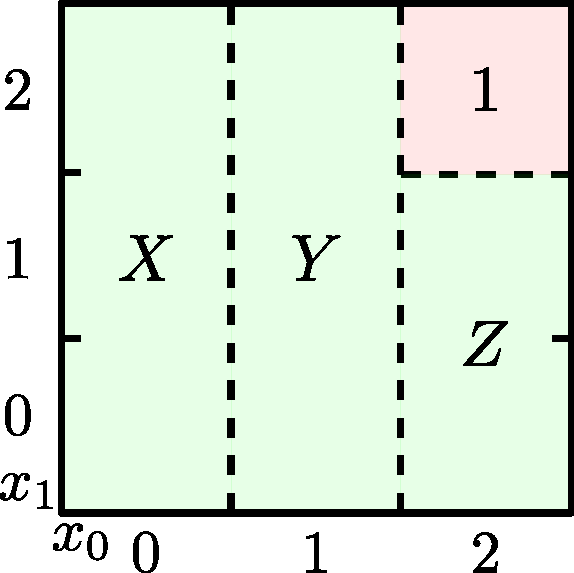
\includegraphics[scale=0.45]{figs/pd_split_thermal.pdf}
    \caption{\textbf{Qutrit phase space regions for $W_{\rho | \tau}(\x)$.}
    Here, the negative component of the magic state overlaps the Wigner distribution of $|0\>$. The rescaled distribution attains a single value in each of the four regions, proportional to the value depicted in the region, see~\cref{eq:bmw_rescaled}.
    }
    \label{fig:pd_split}
\end{figure}

We now denote by $\w(\rho), \w(\rho|\tau)$ the unique values occurring in $W_\rho(\x), W_{\rho|\tau}(\x)$ respectively and $\bmm$ the vector of associated multiplicities of each value in $W_\rho(\x)$. The component values and multiplicities of the relevant distributions in the four distinct regions are given by
\begin{align}
	\w(\rho) &\coloneqq (-v, u, u, u), \\
		\bmm &\coloneqq (1,2,3,3), \\
	\bmw(\tau) &\coloneqq \frac{1}{3\Z} \left( e^{-\beta E_0}, e^{-\beta E_0}, e^{-\beta E_1}, e^{-\beta E_2} \right), \\
	\bmw(\rho_{\rm{S}} | \tau) &\coloneqq 3\Z \left( -v e^{\beta E_0}, u e^{\beta E_0}, u e^{\beta E_1}, u e^{\beta E_2} \right). \label{eq:bmw_rescaled}
\end{align}

Using this notation, the values and multiplicities of the $n$--copy distribution $\bmw(\rho_n |\tau_n)$ are computed in~\cref{lem:ncopycomponents} in~\cref{app:cmpairs}. The values are given by 
\begin{align}\label{eq:ncopy_w_rescaled}
	[\w(\rho_n | \tau_n)]_{ijk} &= (3\Z)^{n} (-v)^{n-\alpha} u^{\alpha} e^{\beta (n-\alpha)E_s} e^{\beta ( i E_0 + j E_1 + k E_2 )},
\end{align}
where the indices $i,j,k$ are non-negative integers that obey the constraint $\alpha \coloneqq i+j+k \leq n$.
The multiplicity of this above value is $m_{ijk}$ with
\begin{equation}
	m_{ijk} = \frac{n!}{i!j!k!(n-\alpha)!} 2^i 3^j 3^k.
\end{equation}
The associated components of $\w(\rho_n)$ are given by
\begin{align}
	[\w(\rho_n)]_{ijk} &= (-v)^{n-\alpha} u^{\alpha}, \label{eq:ncopy_wrho}\\
	[\w(\tau)]_{ijk} &= (3\Z)^{-n} e^{-\beta (n-\alpha)E_s} e^{-\beta ( i E_0 + j E_1 + k E_2 )}. \label{eq:ncopy_wsigma}
\end{align}

In order to construct the $n$--copy Lorenz curve $L_{\rho_n|\tau_n}(x)$ we need to order the components of the distribution, $w(\rho_{\rm{S}} | \tau)_{ijk}$ in decreasing order, and identify the sequence of indices that give us $W_{\rho_n}(\pi(\x))$.

Generally this is complex, but in order to obtain distillation bounds it is sufficient to determine the location of the first elbow $(x_0, L_0)$ of $L_{\rho_n|\tau_n}(\x)$. To do so, we compute the largest component 
\begin{equation}
	w_{\rm max} \coloneqq \max_{i,j,k} [\w(\rho_n | \tau_n)]_{ijk},
\end{equation}
and determine the indices at which this occurs.
Putting in the values we obtain
\begin{align}
	&(3\Z)^{-n}w_{\rm max} = \nonumber\\
	&\max\limits_{i,j,k}\Big\{ (-v)^{n-\alpha} u^{\alpha} e^{\beta (n-\alpha)E_s} e^{\beta ( i E_0 + j E_1 + k E_2 )} \Big\}, \label{eq:max_slope}
\end{align}
where $0 \leq i,j,k \leq n$ and $\alpha \coloneqq i+j+k \leq n$.
Now for $0 \leq \epsilon \leq 3/7$, we have $v \geq u$. Since we assume that $n$ is even, we need the sum $\alpha = i+j+k$ to be even too, so that the expression is positive. 

Given an even value for $\alpha$, the term $v^{n-\alpha} u^{\alpha} e^{-\beta (n-\alpha)E_s}$ is fixed, so the expression is maximised by setting the coefficient of the highest energy $E_{\rm{max}}$ equal to $\alpha$.
Hence, we have
\begin{align}
	&w_{\rm max} = \nonumber\\
	&(3\Z)^{n} v^n e^{n\beta E_s}\max\limits_{\substack{\alpha = 0,2, \\ \dots,n-2,n}}{\Big\{ \left( \frac{u}{v} e^{\beta (E_{\rm{max}} - E_s)} \right)^{\alpha} \Big\}}.
\end{align}
If the expression $\frac{u(\epsilon)}{v(\epsilon)} e^{\beta (E_{\rm{max}} - E_s)}$ is less than $1$ then the maximum occurs at $\alpha=0$, otherwise it occurs at $\alpha = n$. For a fixed state $\tau$, this transition is determined by the value of the depolarising noise parameter $\epsilon$ of the noisy magic state. The transition occurs at $\epsilon = \epsilon_\star$ where
\begin{equation}\label{eq:noise_transition}
	\frac{u(\epsilon_\star)}{v(\epsilon_\star)} e^{\beta (E_{\rm{max}} - E_s)} = \frac{3-\epsilon_\star}{6-8\epsilon_\star} e^{\beta (E_{\rm{max}} - E_s)} = 1.
\end{equation}
If $E_{\rm{max}} = E_s$, namely if the state negativity lies in the same phase space region as the highest energy, this threshold is constant in temperature and given by $\epsilon_{\star} = 3/7$. However, the condition that $\epsilon_\star \ge 0$ also implies a constraint on the effective temperature of the stabilizer state. Specifically, there is a threshold temperature value $\beta_\star$ given by
\begin{equation}
	\beta_{\star} \coloneqq \frac{1}{E_{\rm{max}} - E_s} \ln2,
\end{equation}
such that for the regime $0 \leq \beta \leq \beta_\star$ a transition noise level $\epsilon_\star$ exists, and for $\beta > \beta_\star$ no such transition exists, so we choose $\epsilon_\star = 0$. 
Therefore, the transition value for the noise is given by
\begin{equation}
	\epsilon_{\star}(\beta) \coloneqq 
	\begin{cases}
		3 - \dfrac{9}{4-2^{\beta/\beta_\star - 1}}, &\text{ for } \beta \leq \beta_\star \\
		0, &\text{ for } \beta > \beta_\star.
	\end{cases}
\end{equation}
The quantity $w(\rho_{\rm{S}} | \sigma)_{\rm{max}}$ is now given by
\begin{equation*}
w_{\rm max} =
	\begin{cases}
		(3\Z)^{n} v^n e^{n\beta E_s}, &\mbox{if }\epsilon \leq \epsilon_{\star},\ \hspace{3pt}\rm{(C1)}\\
		(3\Z)^{n} u^n e^{n\beta E_{\rm{max}}}, &\mbox{if }\epsilon > \epsilon_{\star}.\ \hspace{5pt}\rm{(C2)} 
	\end{cases}
\end{equation*}
Case $\rm{(C1)}$ corresponds to $(i,j,k) = (0,0,0)$, so the multiplicity is $m_{000} = 1$, while
Case $\rm{(C2)}$ corresponds to
\begin{equation}
	(i,j,k) = 
	\begin{cases}
	(0,n,0), &\text{if } E_{\rm{max}} = E_1, \\
	(0,0,n), &\text{if } E_{\rm{max}} = E_2,
	\end{cases}
\end{equation}
so the multiplicity in both cases is $3^n$.

Using that $F = -\beta^{-1} \log \Z$, the first elbow coordinates in the two cases are now given by
\begin{equation}\label{eq:first_elb_coords}
	(x_0, L_0) =
	\begin{cases}
		\left(\frac{1}{3^n} e^{-n\beta (E_s - F)}, v^n \right), &\epsilon \leq \epsilon_\star \vspace{10pt}\\
		\left( e^{-n\beta (E_{\rm{max}}-F)}, (3u)^n \right). &\epsilon > \epsilon_\star
	\end{cases}
\end{equation}

\ddd{[Hmmm this needs an additional assumption on the output state to re-run the same analysis. Very annoying.]}\nick{What additional assumption beyond that the output state can be written as a Gibbs state for some $H'$?}
Similarly, considering the output magic state with respect to state $\sigma'$, the image of equilibrium state $\sigma$ under the magic protocol, we get output Lorenz curve coordinates,
\begin{equation}\label{eq:transformed_first_elb_coords}
	(x'_0, L'_0) =
	\begin{cases}
		\left(\frac{1}{3^{n'}} e^{-n\beta (E'_s - F')}, v(\epsilon')^{n'} \right), &\epsilon' \leq \epsilon'_\star \vspace{10pt}\\
		\left( e^{-n'\beta (E'_{\rm{max}}\hspace{-2.5pt}-F')}, (3u(\epsilon'))^{n'} \right), &\epsilon' > \epsilon'_\star
	\end{cases}
\end{equation}
There are four combinations of coordinates, depending on the noise parameters $\epsilon, \epsilon'$ for the input and output states.
In each of these combinations, we simply use the first elbow constraint, as described in~\cref{app:elb_constraints}, which leads to the bounds in the statement of the theorem.
\end{proof}






























\end{document}